% Options for packages loaded elsewhere
\PassOptionsToPackage{unicode}{hyperref}
\PassOptionsToPackage{hyphens}{url}
%
\documentclass[
  ignorenonframetext,
]{beamer}
\usepackage{pgfpages}
\setbeamertemplate{caption}[numbered]
\setbeamertemplate{caption label separator}{: }
\setbeamercolor{caption name}{fg=normal text.fg}
\beamertemplatenavigationsymbolsempty
% Prevent slide breaks in the middle of a paragraph
\widowpenalties 1 10000
\raggedbottom
\setbeamertemplate{part page}{
  \centering
  \begin{beamercolorbox}[sep=16pt,center]{part title}
    \usebeamerfont{part title}\insertpart\par
  \end{beamercolorbox}
}
\setbeamertemplate{section page}{
  \centering
  \begin{beamercolorbox}[sep=12pt,center]{part title}
    \usebeamerfont{section title}\insertsection\par
  \end{beamercolorbox}
}
\setbeamertemplate{subsection page}{
  \centering
  \begin{beamercolorbox}[sep=8pt,center]{part title}
    \usebeamerfont{subsection title}\insertsubsection\par
  \end{beamercolorbox}
}
\AtBeginPart{
  \frame{\partpage}
}
\AtBeginSection{
  \ifbibliography
  \else
    \frame{\sectionpage}
  \fi
}
\AtBeginSubsection{
  \frame{\subsectionpage}
}
\usepackage{amsmath,amssymb}
\usepackage{iftex}
\ifPDFTeX
  \usepackage[T1]{fontenc}
  \usepackage[utf8]{inputenc}
  \usepackage{textcomp} % provide euro and other symbols
\else % if luatex or xetex
  \usepackage{unicode-math} % this also loads fontspec
  \defaultfontfeatures{Scale=MatchLowercase}
  \defaultfontfeatures[\rmfamily]{Ligatures=TeX,Scale=1}
\fi
\usepackage{lmodern}
\usetheme[]{Madrid}
\ifPDFTeX\else
  % xetex/luatex font selection
\fi
% Use upquote if available, for straight quotes in verbatim environments
\IfFileExists{upquote.sty}{\usepackage{upquote}}{}
\IfFileExists{microtype.sty}{% use microtype if available
  \usepackage[]{microtype}
  \UseMicrotypeSet[protrusion]{basicmath} % disable protrusion for tt fonts
}{}
\makeatletter
\@ifundefined{KOMAClassName}{% if non-KOMA class
  \IfFileExists{parskip.sty}{%
    \usepackage{parskip}
  }{% else
    \setlength{\parindent}{0pt}
    \setlength{\parskip}{6pt plus 2pt minus 1pt}}
}{% if KOMA class
  \KOMAoptions{parskip=half}}
\makeatother
\usepackage{xcolor}
\newif\ifbibliography
\usepackage{color}
\usepackage{fancyvrb}
\newcommand{\VerbBar}{|}
\newcommand{\VERB}{\Verb[commandchars=\\\{\}]}
\DefineVerbatimEnvironment{Highlighting}{Verbatim}{commandchars=\\\{\}}
% Add ',fontsize=\small' for more characters per line
\usepackage{framed}
\definecolor{shadecolor}{RGB}{248,248,248}
\newenvironment{Shaded}{\begin{snugshade}}{\end{snugshade}}
\newcommand{\AlertTok}[1]{\textcolor[rgb]{0.94,0.16,0.16}{#1}}
\newcommand{\AnnotationTok}[1]{\textcolor[rgb]{0.56,0.35,0.01}{\textbf{\textit{#1}}}}
\newcommand{\AttributeTok}[1]{\textcolor[rgb]{0.13,0.29,0.53}{#1}}
\newcommand{\BaseNTok}[1]{\textcolor[rgb]{0.00,0.00,0.81}{#1}}
\newcommand{\BuiltInTok}[1]{#1}
\newcommand{\CharTok}[1]{\textcolor[rgb]{0.31,0.60,0.02}{#1}}
\newcommand{\CommentTok}[1]{\textcolor[rgb]{0.56,0.35,0.01}{\textit{#1}}}
\newcommand{\CommentVarTok}[1]{\textcolor[rgb]{0.56,0.35,0.01}{\textbf{\textit{#1}}}}
\newcommand{\ConstantTok}[1]{\textcolor[rgb]{0.56,0.35,0.01}{#1}}
\newcommand{\ControlFlowTok}[1]{\textcolor[rgb]{0.13,0.29,0.53}{\textbf{#1}}}
\newcommand{\DataTypeTok}[1]{\textcolor[rgb]{0.13,0.29,0.53}{#1}}
\newcommand{\DecValTok}[1]{\textcolor[rgb]{0.00,0.00,0.81}{#1}}
\newcommand{\DocumentationTok}[1]{\textcolor[rgb]{0.56,0.35,0.01}{\textbf{\textit{#1}}}}
\newcommand{\ErrorTok}[1]{\textcolor[rgb]{0.64,0.00,0.00}{\textbf{#1}}}
\newcommand{\ExtensionTok}[1]{#1}
\newcommand{\FloatTok}[1]{\textcolor[rgb]{0.00,0.00,0.81}{#1}}
\newcommand{\FunctionTok}[1]{\textcolor[rgb]{0.13,0.29,0.53}{\textbf{#1}}}
\newcommand{\ImportTok}[1]{#1}
\newcommand{\InformationTok}[1]{\textcolor[rgb]{0.56,0.35,0.01}{\textbf{\textit{#1}}}}
\newcommand{\KeywordTok}[1]{\textcolor[rgb]{0.13,0.29,0.53}{\textbf{#1}}}
\newcommand{\NormalTok}[1]{#1}
\newcommand{\OperatorTok}[1]{\textcolor[rgb]{0.81,0.36,0.00}{\textbf{#1}}}
\newcommand{\OtherTok}[1]{\textcolor[rgb]{0.56,0.35,0.01}{#1}}
\newcommand{\PreprocessorTok}[1]{\textcolor[rgb]{0.56,0.35,0.01}{\textit{#1}}}
\newcommand{\RegionMarkerTok}[1]{#1}
\newcommand{\SpecialCharTok}[1]{\textcolor[rgb]{0.81,0.36,0.00}{\textbf{#1}}}
\newcommand{\SpecialStringTok}[1]{\textcolor[rgb]{0.31,0.60,0.02}{#1}}
\newcommand{\StringTok}[1]{\textcolor[rgb]{0.31,0.60,0.02}{#1}}
\newcommand{\VariableTok}[1]{\textcolor[rgb]{0.00,0.00,0.00}{#1}}
\newcommand{\VerbatimStringTok}[1]{\textcolor[rgb]{0.31,0.60,0.02}{#1}}
\newcommand{\WarningTok}[1]{\textcolor[rgb]{0.56,0.35,0.01}{\textbf{\textit{#1}}}}
\usepackage{graphicx}
\makeatletter
\def\maxwidth{\ifdim\Gin@nat@width>\linewidth\linewidth\else\Gin@nat@width\fi}
\def\maxheight{\ifdim\Gin@nat@height>\textheight\textheight\else\Gin@nat@height\fi}
\makeatother
% Scale images if necessary, so that they will not overflow the page
% margins by default, and it is still possible to overwrite the defaults
% using explicit options in \includegraphics[width, height, ...]{}
\setkeys{Gin}{width=\maxwidth,height=\maxheight,keepaspectratio}
% Set default figure placement to htbp
\makeatletter
\def\fps@figure{htbp}
\makeatother
\setlength{\emergencystretch}{3em} % prevent overfull lines
\providecommand{\tightlist}{%
  \setlength{\itemsep}{0pt}\setlength{\parskip}{0pt}}
\setcounter{secnumdepth}{-\maxdimen} % remove section numbering
\ifLuaTeX
  \usepackage{selnolig}  % disable illegal ligatures
\fi
\usepackage{bookmark}
\IfFileExists{xurl.sty}{\usepackage{xurl}}{} % add URL line breaks if available
\urlstyle{same}
\hypersetup{
  pdftitle={Trajnim Themelor Microsoft 365},
  hidelinks,
  pdfcreator={LaTeX via pandoc}}

\title{Trajnim Themelor Microsoft 365}
\subtitle{Gjithçka për punën e përditshme}
\author{}
\date{\vspace{-2.5em}17 December, 2024}

\begin{document}
\frame{\titlepage}

\begin{frame}[allowframebreaks]
  \tableofcontents[hideallsubsections]
\end{frame}
\section{Microsoft 365 Word}\label{microsoft-365-word}

\begin{frame}{Hyrje në Word Online}
\phantomsection\label{hyrje-nuxeb-word-online}
\begin{itemize}
\item
  \textbf{Microsoft Word Web} është një version online i Word-it në
  \textbf{Office 365}.
\item
  Ju mund të:

  \begin{itemize}
  \item
    Krijoni dhe redaktoni dokumente direkt nga një shfletues web.
  \item
    Ruani punën tuaj automatikisht në \textbf{OneDrive}.
  \item
    Bashkëpunoni në kohë reale me të tjerët.
  \end{itemize}
\end{itemize}
\end{frame}

\begin{frame}{Hyrja në Office 365}
\phantomsection\label{hyrja-nuxeb-office-365}
\begin{enumerate}
\item
  Hapni shfletuesin tuaj dhe shkoni te:

  \textbf{\url{https://www.office.com}}
\item
  Identifikohuni me kredencialet tuaja të \textbf{Microsoft 365}.
\end{enumerate}
\end{frame}

\begin{frame}{Hyrja në Office 365}
\phantomsection\label{hyrja-nuxeb-office-365-1}
\begin{enumerate}
\setcounter{enumi}{2}
\tightlist
\item
  Nga paneli kryesor, klikoni mbi ikonën \textbf{Word} (ikonë blu me W
  të bardhë).
\end{enumerate}

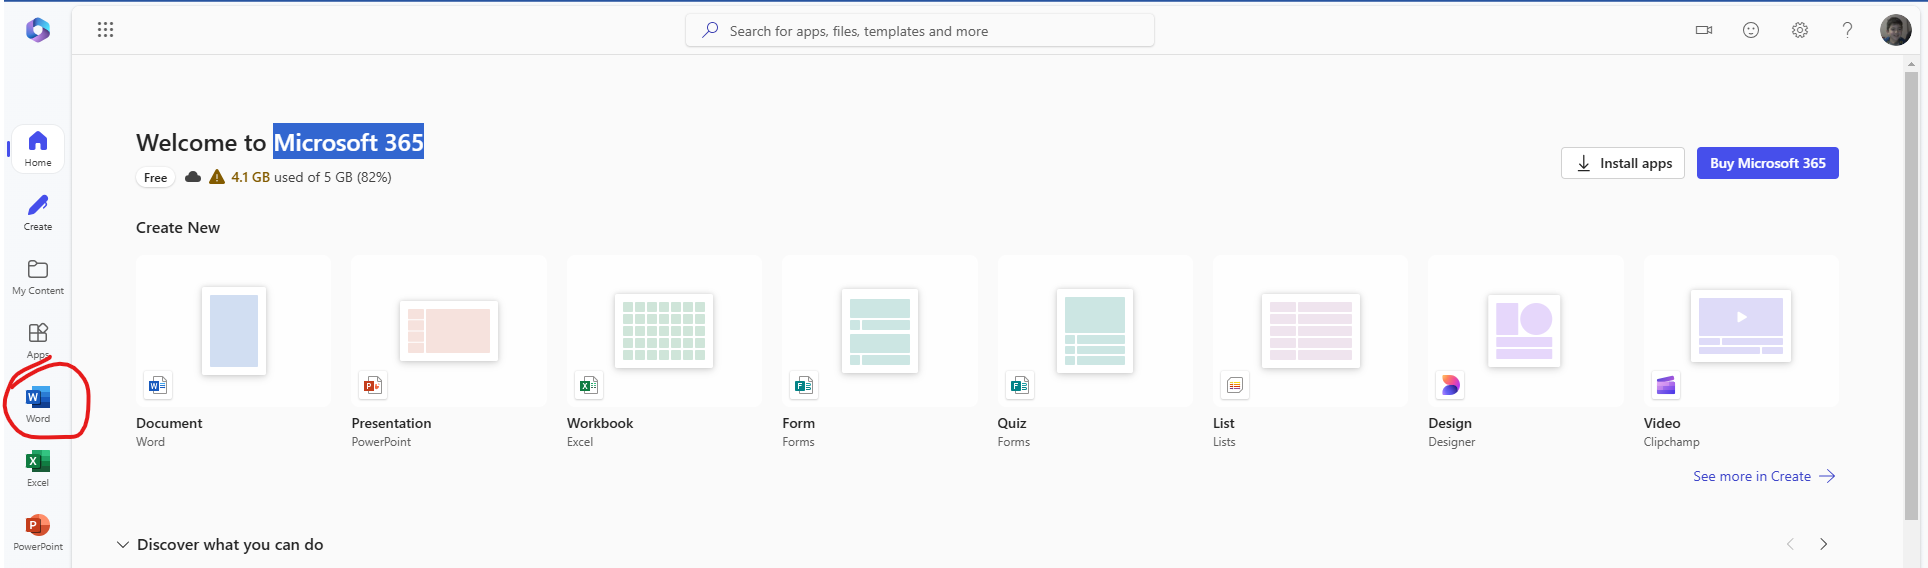
\includegraphics{./images/word1.png}
\end{frame}

\begin{frame}{Krijimi i një dokumenti të ri}
\phantomsection\label{krijimi-i-njuxeb-dokumenti-tuxeb-ri}
\begin{enumerate}
\item
  Pasi të hapet Word Online, klikoni mbi \textbf{``New Blank Document''}
  (Dokument i Ri).
\item
  Mund të zgjidhni edhe një \textbf{template} (model) për dokumente të
  parapërgatitura.
\end{enumerate}

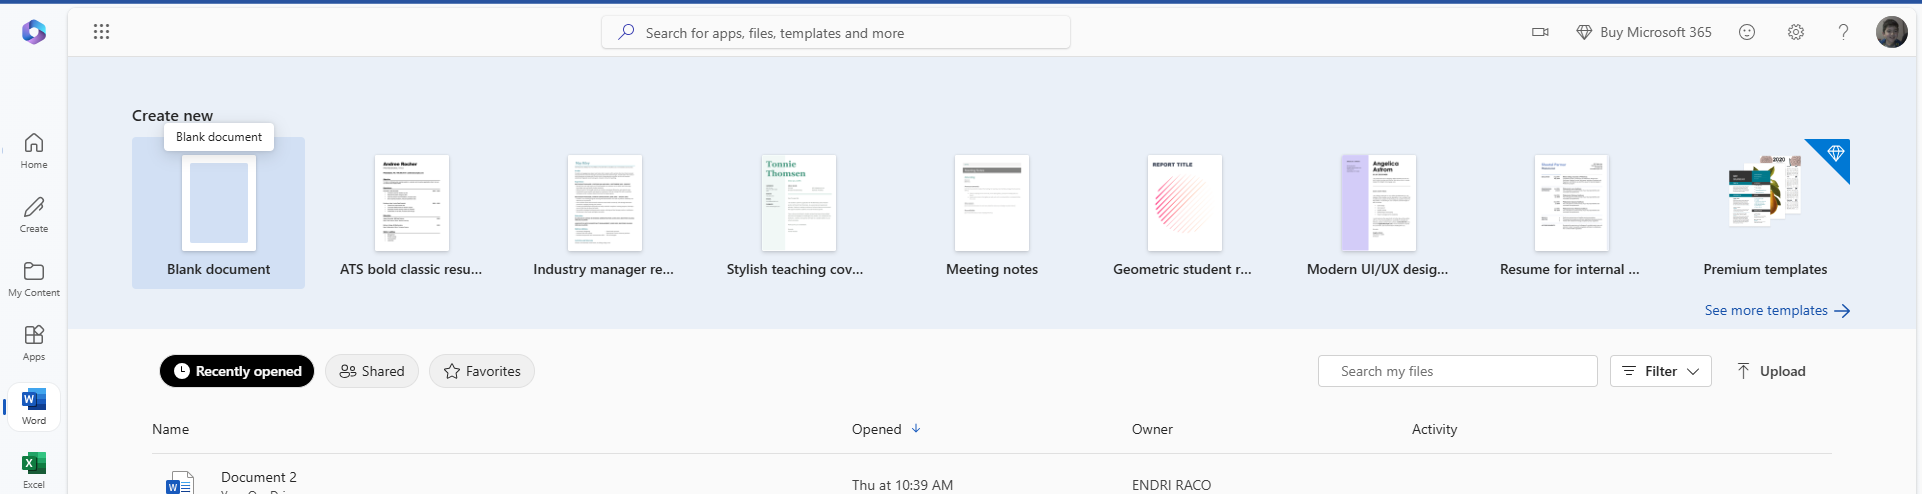
\includegraphics{./images/word2.png}
\end{frame}

\begin{frame}{Ndërfaqja e Word Web}
\phantomsection\label{nduxebrfaqja-e-word-web}
Pjesët kryesore të ndërfaqes:

\begin{enumerate}
\item
  \textbf{Ribbon}: Përmban mjetet e redaktimit (Home, Insert, Layout,
  etj.).
\item
  \textbf{Document Area}: Hapësira ku shkruani përmbajtjen tuaj.
\item
  \textbf{AutoSave}: Dokumenti ruhet automatikisht në \textbf{OneDrive}.
\item
  \textbf{Share}: Opsion për të ndarë dokumentin me të tjerët.
\end{enumerate}
\end{frame}

\begin{frame}{Ndërfaqja e Word Web}
\phantomsection\label{nduxebrfaqja-e-word-web-1}
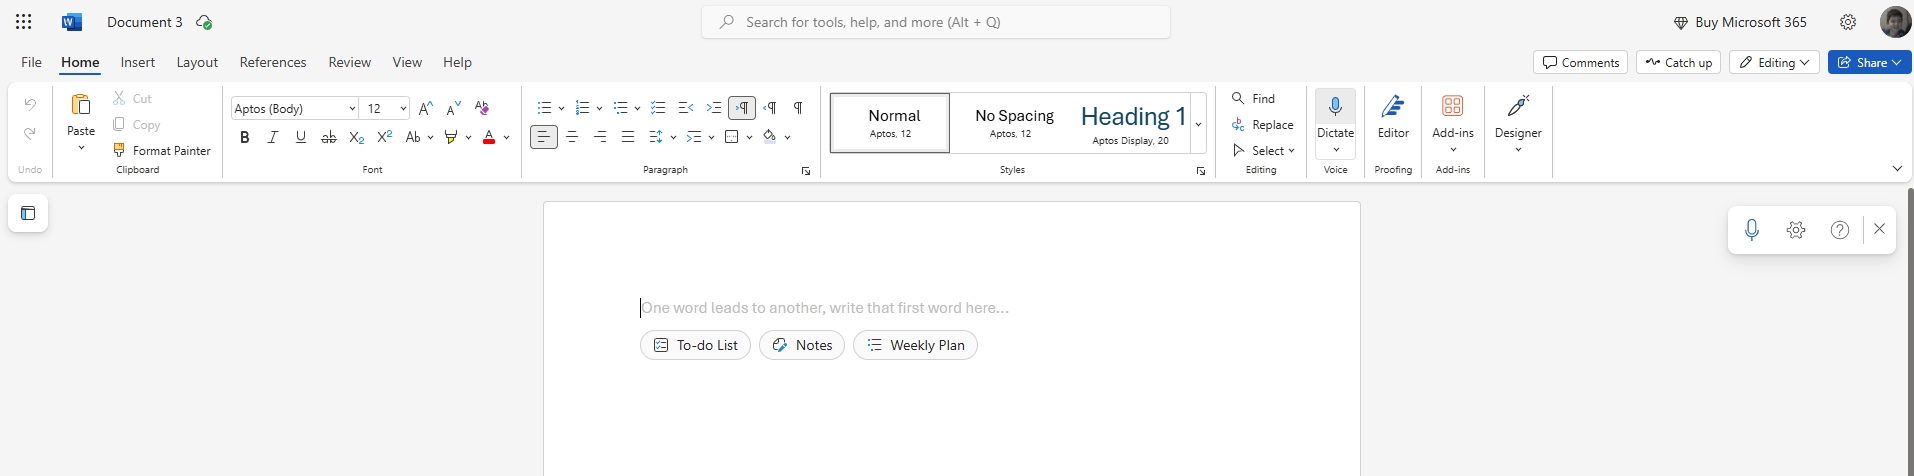
\includegraphics{./images/word3.png}
\end{frame}

\begin{frame}{Redaktimi i përmbajtjes}
\phantomsection\label{redaktimi-i-puxebrmbajtjes}
\begin{enumerate}
\item
  \textbf{Shkrimi i tekstit}: Klikoni në dokument dhe filloni të
  shkruani.
\item
  \textbf{Formatimi i tekstit}:

  \begin{itemize}
  \item
    Përdorni seksionin \textbf{Home} për të:

    \begin{itemize}
    \item
      Ndryshuar fontin, madhësinë, dhe ngjyrën e tekstit.
    \item
      Vendosur bold (\textbf{B}), italic (\emph{I}), ose underline
      (\textbf{U}).
    \end{itemize}
  \end{itemize}
\end{enumerate}
\end{frame}

\begin{frame}{Redaktimi i përmbajtjes}
\phantomsection\label{redaktimi-i-puxebrmbajtjes-1}
\begin{enumerate}
\setcounter{enumi}{2}
\item
  \textbf{Shtimi i listave dhe numërimeve}:

  \begin{itemize}
  \tightlist
  \item
    Zgjidhni tekstin dhe përdorni opsionet për \textbf{bullets} ose
    \textbf{numbering}.
  \end{itemize}
\end{enumerate}

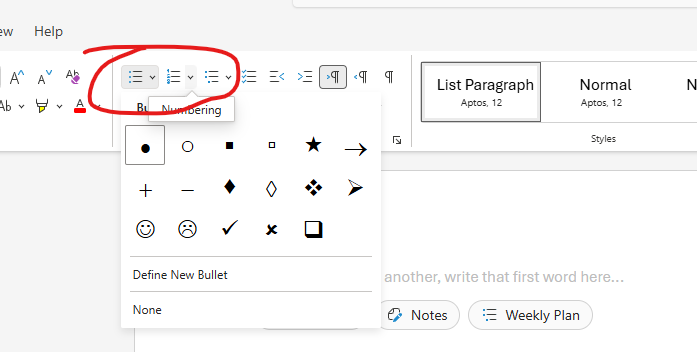
\includegraphics{./images/word4.png}
\end{frame}

\begin{frame}{Shtimi i elementeve të tjera}
\phantomsection\label{shtimi-i-elementeve-tuxeb-tjera}
\begin{enumerate}
\item
  Shkoni te seksioni \textbf{Insert} në Ribbon për të:

  \begin{itemize}
  \item
    \textbf{Shtuar imazhe} nga kompjuteri ose interneti.
  \item
    \textbf{Krijuar tabela} për të organizuar informacionin.
  \item
    \textbf{Vendosur lidhje (Links)} për të shtuar hyperlink.
  \end{itemize}
\end{enumerate}
\end{frame}

\begin{frame}{Shtimi i elementeve të tjera}
\phantomsection\label{shtimi-i-elementeve-tuxeb-tjera-1}
\begin{enumerate}
\setcounter{enumi}{1}
\tightlist
\item
  Përdorni \textbf{Header dhe Footer} për të shtuar tituj dhe numra
  faqe.
\end{enumerate}

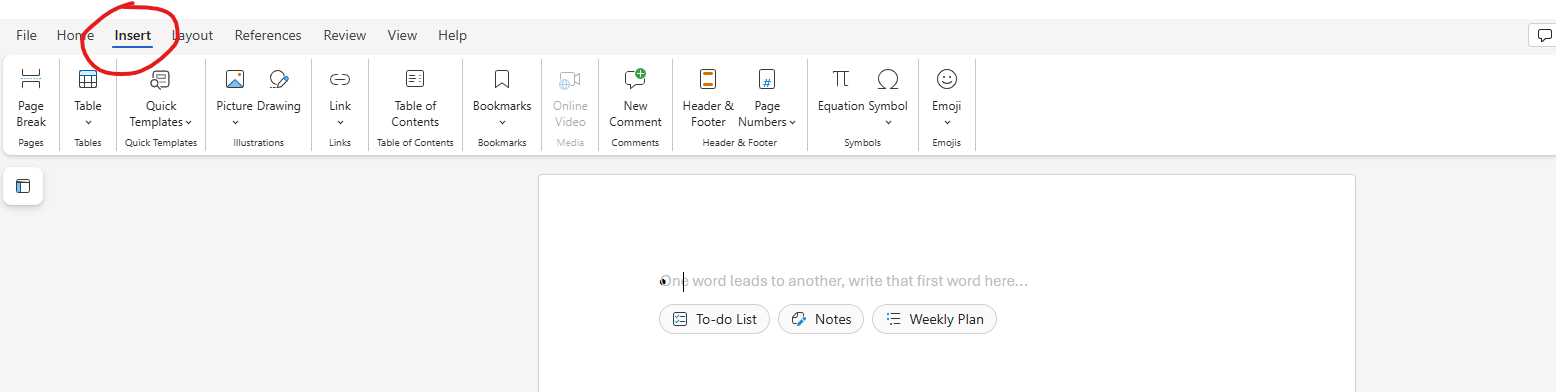
\includegraphics{./images/word5.png}
\end{frame}

\begin{frame}{Bashkëpunimi në dokument}
\phantomsection\label{bashkuxebpunimi-nuxeb-dokument}
\begin{enumerate}
\item
  Klikoni mbi butonin \textbf{``Share''} në të djathtë të ekranit.
\item
  Ftoni të tjerët duke vendosur adresën e email-it të tyre.
\item
  Zgjidhni lejet:

  \begin{itemize}
  \item
    \textbf{Can edit}: Përdoruesit mund të bëjnë ndryshime.
  \item
    \textbf{Can view}: Përdoruesit mund të shohin vetëm dokumentin.
  \end{itemize}
\end{enumerate}
\end{frame}

\begin{frame}{Bashkëpunimi në dokument}
\phantomsection\label{bashkuxebpunimi-nuxeb-dokument-1}
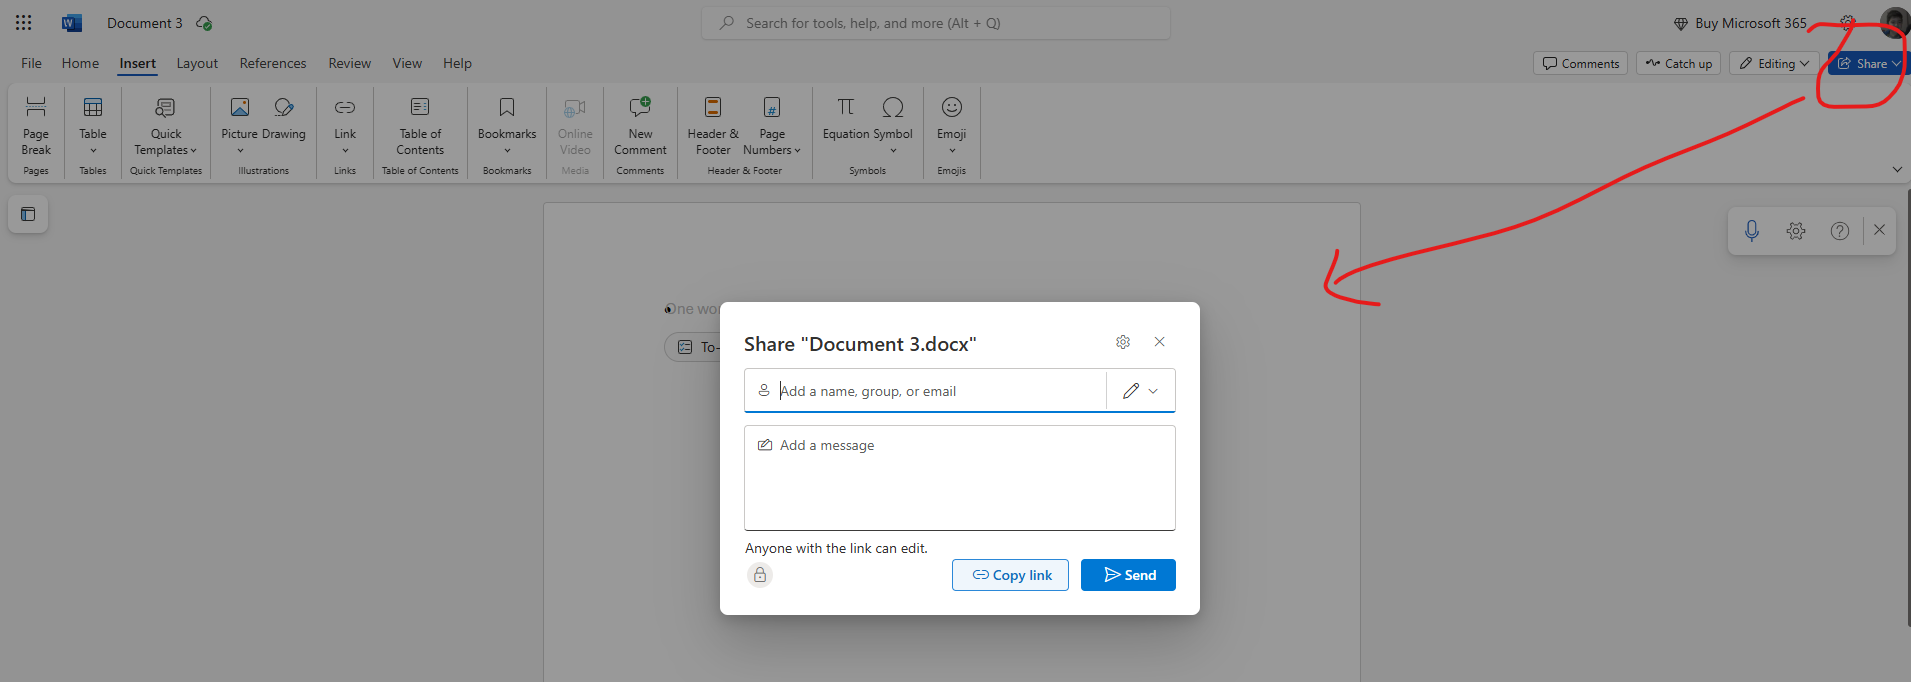
\includegraphics{./images/word6.png}
\end{frame}

\begin{frame}{Ruajtja dhe eksportimi i dokumentit}
\phantomsection\label{ruajtja-dhe-eksportimi-i-dokumentit}
\begin{enumerate}
\item
  Dokumenti juaj ruhet automatikisht në \textbf{OneDrive}.
\item
  Për të shkarkuar dokumentin:

  \begin{itemize}
  \tightlist
  \item
    Klikoni mbi \textbf{File} \textgreater{} \textbf{Save As}
    \textgreater{} \textbf{Download a Copy}.
  \end{itemize}
\end{enumerate}
\end{frame}

\begin{frame}{Ruajtja dhe eksportimi i dokumentit}
\phantomsection\label{ruajtja-dhe-eksportimi-i-dokumentit-1}
\begin{enumerate}
\setcounter{enumi}{2}
\item
  Mund ta eksportoni si:

  \begin{itemize}
  \item
    \textbf{Word (.docx)}
  \item
    \textbf{PDF}.
  \end{itemize}
\end{enumerate}

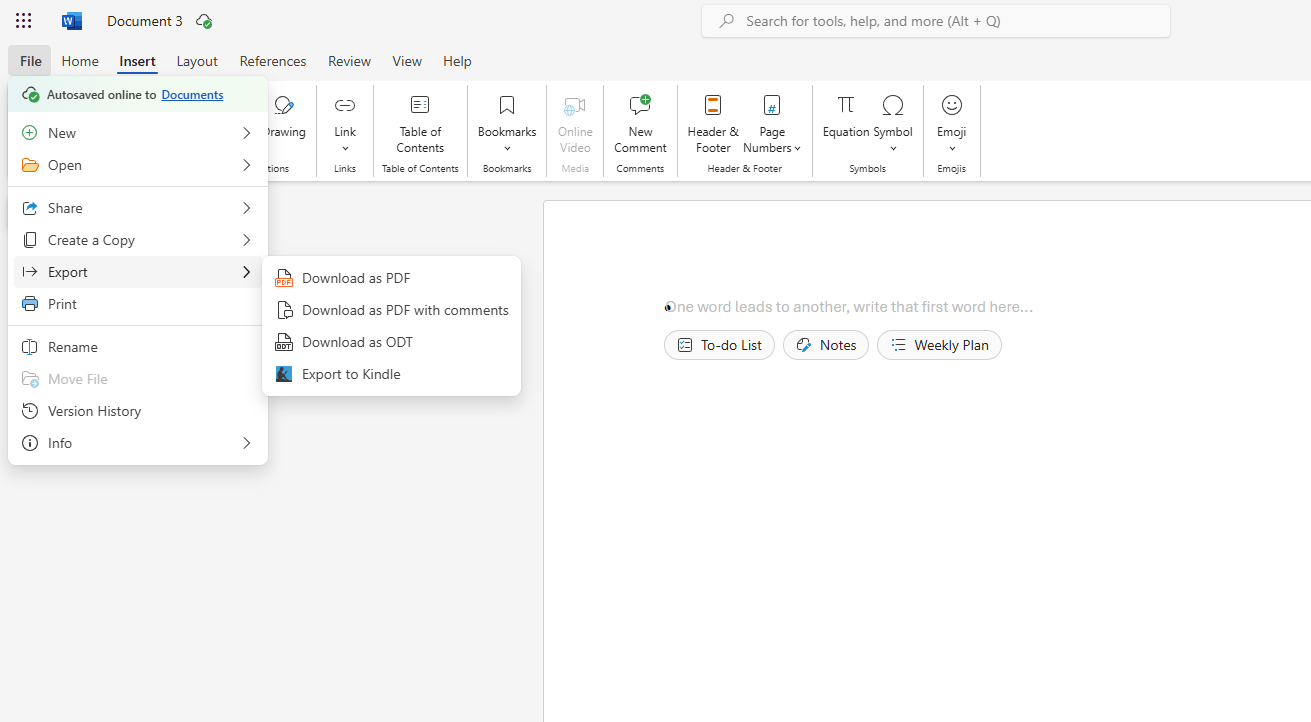
\includegraphics{./images/word7.png}
\end{frame}

\begin{frame}{Përfitimet e përdorimit të Word Web}
\phantomsection\label{puxebrfitimet-e-puxebrdorimit-tuxeb-word-web}
\begin{itemize}
\item
  \textbf{Akses kudo}: Punoni nga çdo pajisje me një lidhje interneti.
\item
  \textbf{AutoSave}: Dokumenti ruhet automatikisht në cloud.
\item
  \textbf{Bashkëpunim në kohë reale}: Redaktoni dokumentin njëkohësisht
  me të tjerët.
\item
  \textbf{Pa instalim}: Nuk kërkohet asnjë softuer shtesë.
\end{itemize}
\end{frame}

\begin{frame}{Rezultate}
\phantomsection\label{rezultate}
\begin{itemize}
\item
  \textbf{Microsoft Word Web} është një mjet i fuqishëm për krijimin dhe
  redaktimin e dokumenteve në mënyrë të shpejtë dhe të thjeshtë.
\item
  Përdorni funksionalitetet si \textbf{formatimi}, \textbf{Insert}, dhe
  \textbf{Share} për të maksimizuar përfitimet e punës suaj.
\end{itemize}
\end{frame}

\begin{frame}{Pyetje \& Diskutim}
\phantomsection\label{pyetje-diskutim}
\begin{itemize}
\tightlist
\item
  A keni përdorur më parë Word Web?
\end{itemize}
\end{frame}

\begin{frame}{Shtimi dhe Redaktimi i Tekstit}
\phantomsection\label{shtimi-dhe-redaktimi-i-tekstit}
\begin{enumerate}
\item
  \textbf{Shtimi i tekstit}:

  \begin{itemize}
  \tightlist
  \item
    Klikoni në hapësirën e dokumentit dhe filloni të shkruani.
  \end{itemize}
\item
  \textbf{Redaktimi i tekstit}:

  \begin{itemize}
  \item
    Zgjidhni tekstin për të ndryshuar fontin, madhësinë dhe ngjyrën.
  \item
    Përdorni opsionet nga menyja \textbf{Home}.
  \end{itemize}
\end{enumerate}
\end{frame}

\begin{frame}{Shtimi dhe Redaktimi i Tekstit}
\phantomsection\label{shtimi-dhe-redaktimi-i-tekstit-1}
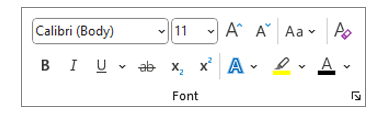
\includegraphics{./images/word19.png}
\end{frame}

\begin{frame}{Gjetja dhe Zëvendësimi i Tekstit}
\phantomsection\label{gjetja-dhe-zuxebvenduxebsimi-i-tekstit}
\begin{enumerate}
\item
  Klikoni mbi \textbf{Home \textgreater{} Find} për të gjetur tekst
  specifik.
\item
  Zgjidhni \textbf{Replace} për të zëvendësuar tekstin me një tjetër.
\end{enumerate}

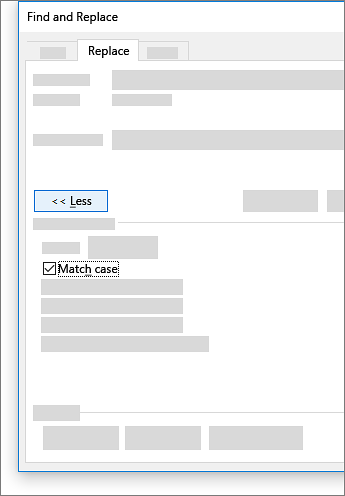
\includegraphics{./images/word20.png}
\end{frame}

\begin{frame}{Kontrolli i Gramatikës dhe Spelling-ut}
\phantomsection\label{kontrolli-i-gramatikuxebs-dhe-spelling-ut}
\begin{enumerate}
\item
  Nga menyja \textbf{Review}, aktivizoni:

  \begin{itemize}
  \tightlist
  \item
    \textbf{Spelling \& Grammar} për të korrigjuar gabimet.
  \end{itemize}
\item
  Word do të sugjerojë korrigjimet për gabimet e shkrimit dhe
  gramatikës.
\end{enumerate}
\end{frame}

\begin{frame}{Kontrolli i Gramatikës dhe Spelling-ut}
\phantomsection\label{kontrolli-i-gramatikuxebs-dhe-spelling-ut-1}
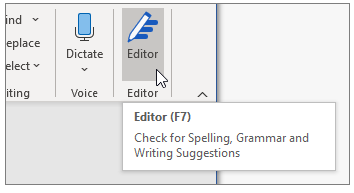
\includegraphics{./images/word21.png}
\end{frame}

\begin{frame}{Shfaqja e Numrit të Fjalëve}
\phantomsection\label{shfaqja-e-numrit-tuxeb-fjaluxebve}
\begin{itemize}
\item
  Klikoni mbi numrin në fund të djathtë të faqes për të parë:

  \begin{itemize}
  \item
    \textbf{Numrin e fjalëve}
  \item
    \textbf{Numrin e karaktereve dhe faqeve}.
  \end{itemize}
\end{itemize}
\end{frame}

\begin{frame}{Shfaqja e Numrit të Fjalëve}
\phantomsection\label{shfaqja-e-numrit-tuxeb-fjaluxebve-1}
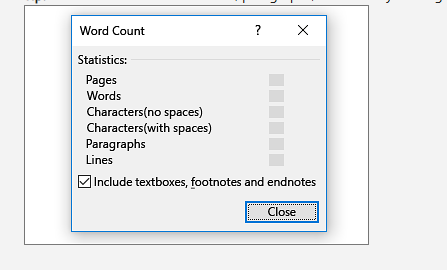
\includegraphics{./images/word22.png}
\end{frame}

\begin{frame}{Formatimi i Tekstit dhe Dokumentit}
\phantomsection\label{formatimi-i-tekstit-dhe-dokumentit}
\begin{enumerate}
\item
  \textbf{Formatimi i Tekstit}:

  \begin{itemize}
  \tightlist
  \item
    Bold (\textbf{B}), Italic (\emph{I}), Underline (\textbf{U}), Font
    dhe madhësi.
  \end{itemize}
\item
  \textbf{Faqosja e Dokumentit}:

  \begin{itemize}
  \item
    Nga menyja \textbf{Layout}, mund të ndryshoni:

    \begin{itemize}
    \item
      \textbf{Margins} (kufijtë)
    \item
      \textbf{Orientation} (Portret ose Peizazh).
    \end{itemize}
  \end{itemize}
\end{enumerate}
\end{frame}

\begin{frame}{Formatimi i Tekstit dhe Dokumentit}
\phantomsection\label{formatimi-i-tekstit-dhe-dokumentit-1}
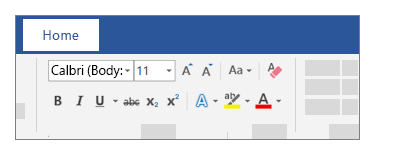
\includegraphics{./images/word23.png}
\end{frame}

\begin{frame}{Futja e Tabelave, Figurave dhe Watermarks}
\phantomsection\label{futja-e-tabelave-figurave-dhe-watermarks}
\begin{enumerate}
\item
  \textbf{Tabelat}:

  \begin{itemize}
  \tightlist
  \item
    \textbf{Insert \textgreater{} Table} për të krijuar tabela.
  \end{itemize}
\item
  \textbf{Figurat}:

  \begin{itemize}
  \tightlist
  \item
    \textbf{Insert \textgreater{} Pictures} për të ngarkuar imazhe.
  \end{itemize}
\item
  \textbf{Watermarks}:

  \begin{itemize}
  \tightlist
  \item
    Nuk mbështetet plotësisht në Word Web, por mund të bëhet në Word
    Desktop.
  \end{itemize}
\end{enumerate}
\end{frame}

\begin{frame}{Futja e Tabelave, Figurave dhe Watermarks}
\phantomsection\label{futja-e-tabelave-figurave-dhe-watermarks-1}
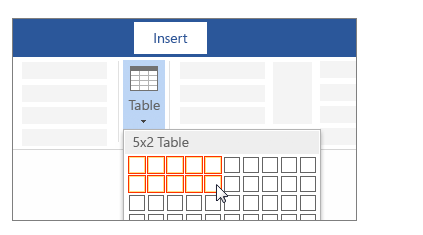
\includegraphics{./images/word24.png}
\end{frame}

\begin{frame}{Ruajtja, Printimi dhe Ndërveprimi me të Tjerët}
\phantomsection\label{ruajtja-printimi-dhe-nduxebrveprimi-me-tuxeb-tjeruxebt}
\begin{enumerate}
\item
  \textbf{Ruajtja}: Dokumenti ruhet automatikisht në \textbf{OneDrive}.
\item
  \textbf{Printimi}: Klikoni \textbf{File \textgreater{} Print} për të
  printuar.
\item
  \textbf{Ndërveprimi}:

  \begin{itemize}
  \tightlist
  \item
    Klikoni \textbf{Share} për të ftuar të tjerët të bashkëpunojnë.
  \end{itemize}
\end{enumerate}
\end{frame}

\begin{frame}{Ruajtja, Printimi dhe Ndërveprimi me të Tjerët}
\phantomsection\label{ruajtja-printimi-dhe-nduxebrveprimi-me-tuxeb-tjeruxebt-1}
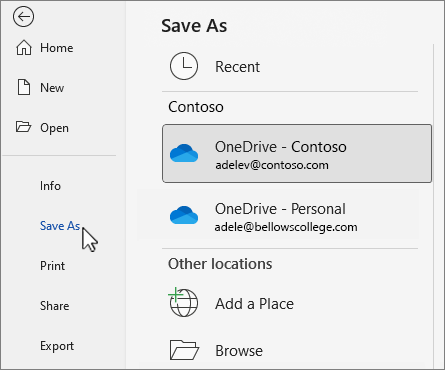
\includegraphics{./images/word25.png}
\end{frame}

\begin{frame}{Si të futni dhe redaktoni Hyperlink-e në Microsoft Word}
\phantomsection\label{si-tuxeb-futni-dhe-redaktoni-hyperlink-e-nuxeb-microsoft-word}
\begin{itemize}
\item
  \textbf{Hyperlink} është një lidhje që ju çon te një faqe interneti,
  skedar ose vendndodhje tjetër në dokument.
\item
  Hyperlink-et janë të dobishme për:

  \begin{itemize}
  \item
    Referenca të jashtme (faqe interneti, artikuj).
  \item
    Lëvizje brenda dokumentit (në seksione ose faqe të tjera).
  \item
    Akses të shpejtë në skedarë dhe materiale mbështetëse.
  \end{itemize}
\end{itemize}
\end{frame}

\begin{frame}{Futja e një Hyperlink në Word Web}
\phantomsection\label{futja-e-njuxeb-hyperlink-nuxeb-word-web}
\begin{enumerate}
\item
  Hapni dokumentin tuaj në \textbf{Word Online} përmes
  \url{https://www.office.com}.
\item
  Zgjidhni tekstin ose objektin që dëshironi të ktheni në një
  \textbf{hyperlink}.
\end{enumerate}
\end{frame}

\begin{frame}{Futja e një Hyperlink në Word Web}
\phantomsection\label{futja-e-njuxeb-hyperlink-nuxeb-word-web-1}
\begin{enumerate}
\setcounter{enumi}{2}
\tightlist
\item
  Klikoni mbi butonin \textbf{Insert} në Ribbon.
\end{enumerate}

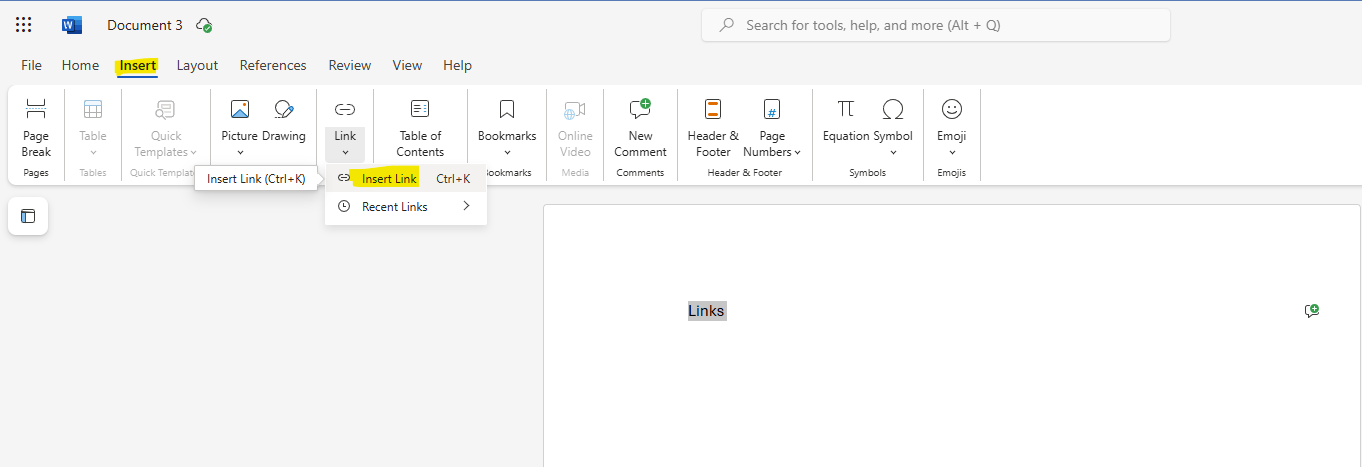
\includegraphics{./images/word8.png}
\end{frame}

\begin{frame}{Futja e një Hyperlink në Word Web}
\phantomsection\label{futja-e-njuxeb-hyperlink-nuxeb-word-web-2}
\begin{enumerate}
\setcounter{enumi}{3}
\item
  Zgjidhni \textbf{Link} (Lidhje) ose shtypni \textbf{Ctrl+K}.
\item
  Në kutinë që shfaqet:

  \begin{itemize}
  \item
    Vendosni URL-në në fushën \textbf{Address} (Adresa).
  \item
    Klikoni \textbf{Insert} (Fut).
  \end{itemize}
\end{enumerate}

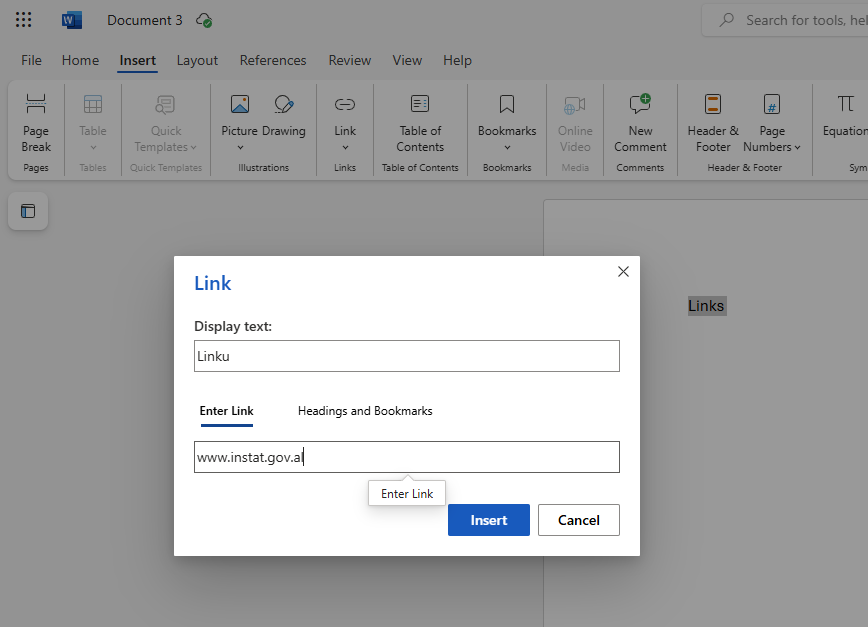
\includegraphics{./images/word9.png}
\end{frame}

\begin{frame}{Redaktimi i një Hyperlink}
\phantomsection\label{redaktimi-i-njuxeb-hyperlink}
\begin{enumerate}
\item
  Klikoni me të djathtën mbi \textbf{hyperlink}-un ekzistues.
\item
  Zgjidhni \textbf{Edit Link} (Redakto Lidhjen).
\end{enumerate}

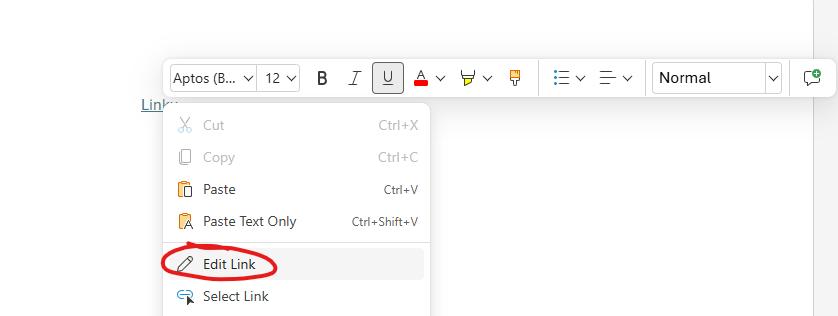
\includegraphics{./images/word11.png}
\end{frame}

\begin{frame}{Redaktimi i një Hyperlink}
\phantomsection\label{redaktimi-i-njuxeb-hyperlink-1}
\begin{enumerate}
\setcounter{enumi}{2}
\item
  Bëni ndryshimet në \textbf{Address} ose ndryshoni tekstin e shfaqur.
\item
  Klikoni \textbf{OK} për të aplikuar ndryshimet.
\end{enumerate}
\end{frame}

\begin{frame}{Fshirja e një Hyperlink}
\phantomsection\label{fshirja-e-njuxeb-hyperlink}
\begin{enumerate}
\item
  Klikoni me të djathtën mbi \textbf{hyperlink}-un.
\item
  Zgjidhni \textbf{Remove Link} (Hiq Lidhjen).
\end{enumerate}
\end{frame}

\begin{frame}{Fshirja e një Hyperlink}
\phantomsection\label{fshirja-e-njuxeb-hyperlink-1}
\begin{enumerate}
\setcounter{enumi}{2}
\tightlist
\item
  Teksti mbetet, por lidhja hiqet.
\end{enumerate}

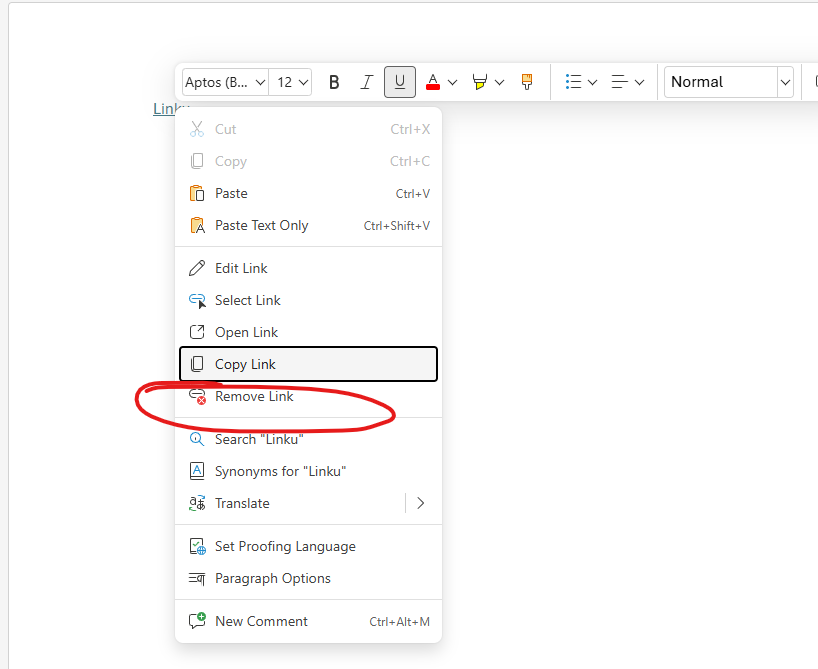
\includegraphics{./images/word12.png}
\end{frame}

\begin{frame}{Këshilla për përdorimin e Hyperlink-eve}
\phantomsection\label{kuxebshilla-puxebr-puxebrdorimin-e-hyperlink-eve}
\begin{itemize}
\item
  Përdorni \textbf{tekste të qarta dhe përshkruese} për hyperlink-et
  (p.sh., ``Klikoni këtu për detaje'' nuk është aq i qartë sa ``Lexoni
  udhëzuesin në faqen zyrtare'').
\item
  Kontrolloni gjithmonë që \textbf{URL-të} janë të sakta dhe
  funksionale.
\item
  Përdorni \textbf{hyperlink-e të brendshme} për të përmirësuar
  navigimin brenda dokumentit tuaj.
\end{itemize}
\end{frame}

\begin{frame}{Përfitimet e përdorimit të Hyperlink-eve}
\phantomsection\label{puxebrfitimet-e-puxebrdorimit-tuxeb-hyperlink-eve}
\begin{itemize}
\item
  \textbf{Efikasitet}: Kaloni shpejt nga një dokument në një tjetër ose
  në një faqe interneti.
\item
  \textbf{Bashkëpunim}: Ndani referenca dhe skedarë me bashkëpunëtorët.
\item
  \textbf{Organizim}: Lidhni seksione të rëndësishme brenda të njëjtit
  dokument.
\end{itemize}
\end{frame}

\begin{frame}{Rezultate}
\phantomsection\label{rezultate-1}
\begin{itemize}
\tightlist
\item
  Futja dhe redaktimi i \textbf{hyperlink-eve} në Microsoft Word është e
  thjeshtë dhe ndihmon për ta bërë dokumentin tuaj më funksional dhe të
  organizuar.
\end{itemize}
\end{frame}

\begin{frame}{Pyetje \& Diskutim}
\phantomsection\label{pyetje-diskutim-1}
\begin{itemize}
\tightlist
\item
  Cilat lloje të hyperlink-eve përdorni më shpesh në dokumentet tuaja?
\end{itemize}
\end{frame}

\begin{frame}{Si të futni dhe redaktoni një Footnote në Word Web}
\phantomsection\label{si-tuxeb-futni-dhe-redaktoni-njuxeb-footnote-nuxeb-word-web}
\begin{itemize}
\item
  \textbf{Footnote} është një shënim që shfaqet në fund të faqes për të
  ofruar referenca shtesë ose shpjegime.
\item
  Funksionet e \textbf{footnotes} janë të dobishme për:

  \begin{itemize}
  \item
    Referenca akademike.
  \item
    Shënime plotësuese për tekstin.
  \item
    Burime të caktuara.
  \end{itemize}
\end{itemize}
\end{frame}

\begin{frame}{Vendosja e një Footnote}
\phantomsection\label{vendosja-e-njuxeb-footnote}
\begin{enumerate}
\item
  Klikoni në \textbf{vendi} ku dëshironi të shtoni një footnote në
  dokument.
\item
  Nga menyja në krye (Ribbon), zgjidhni:

  \begin{itemize}
  \tightlist
  \item
    \textbf{References} (Referenca) \textgreater{} \textbf{Insert
    Footnote}.
  \end{itemize}
\end{enumerate}
\end{frame}

\begin{frame}{Vendosja e një Footnote}
\phantomsection\label{vendosja-e-njuxeb-footnote-1}
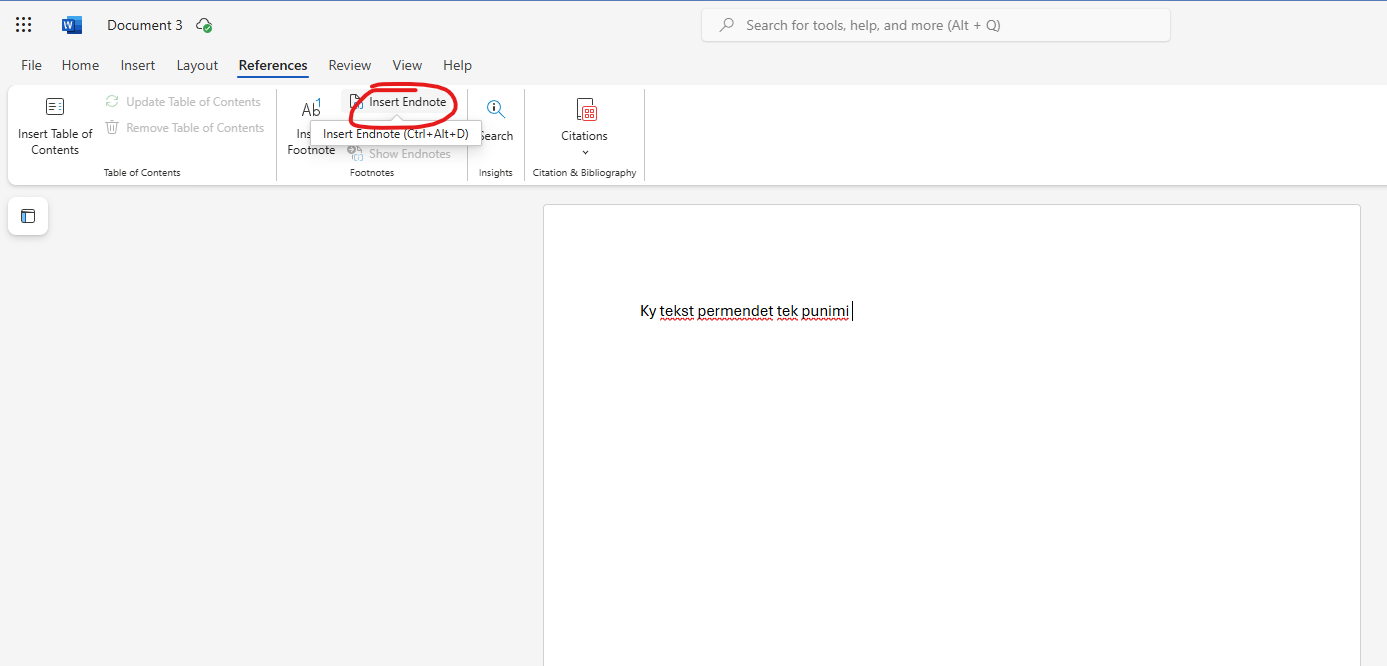
\includegraphics{./images/word13.png}
\end{frame}

\begin{frame}{Vendosja e një Footnote}
\phantomsection\label{vendosja-e-njuxeb-footnote-2}
\begin{enumerate}
\setcounter{enumi}{2}
\item
  Në fund të faqes, do të shfaqet një numër dhe fusha për të shtuar
  shënimin tuaj.
\item
  Shkruani përmbajtjen e \textbf{footnote} në atë fushë.
\end{enumerate}
\end{frame}

\begin{frame}{Vendosja e një Footnote}
\phantomsection\label{vendosja-e-njuxeb-footnote-3}
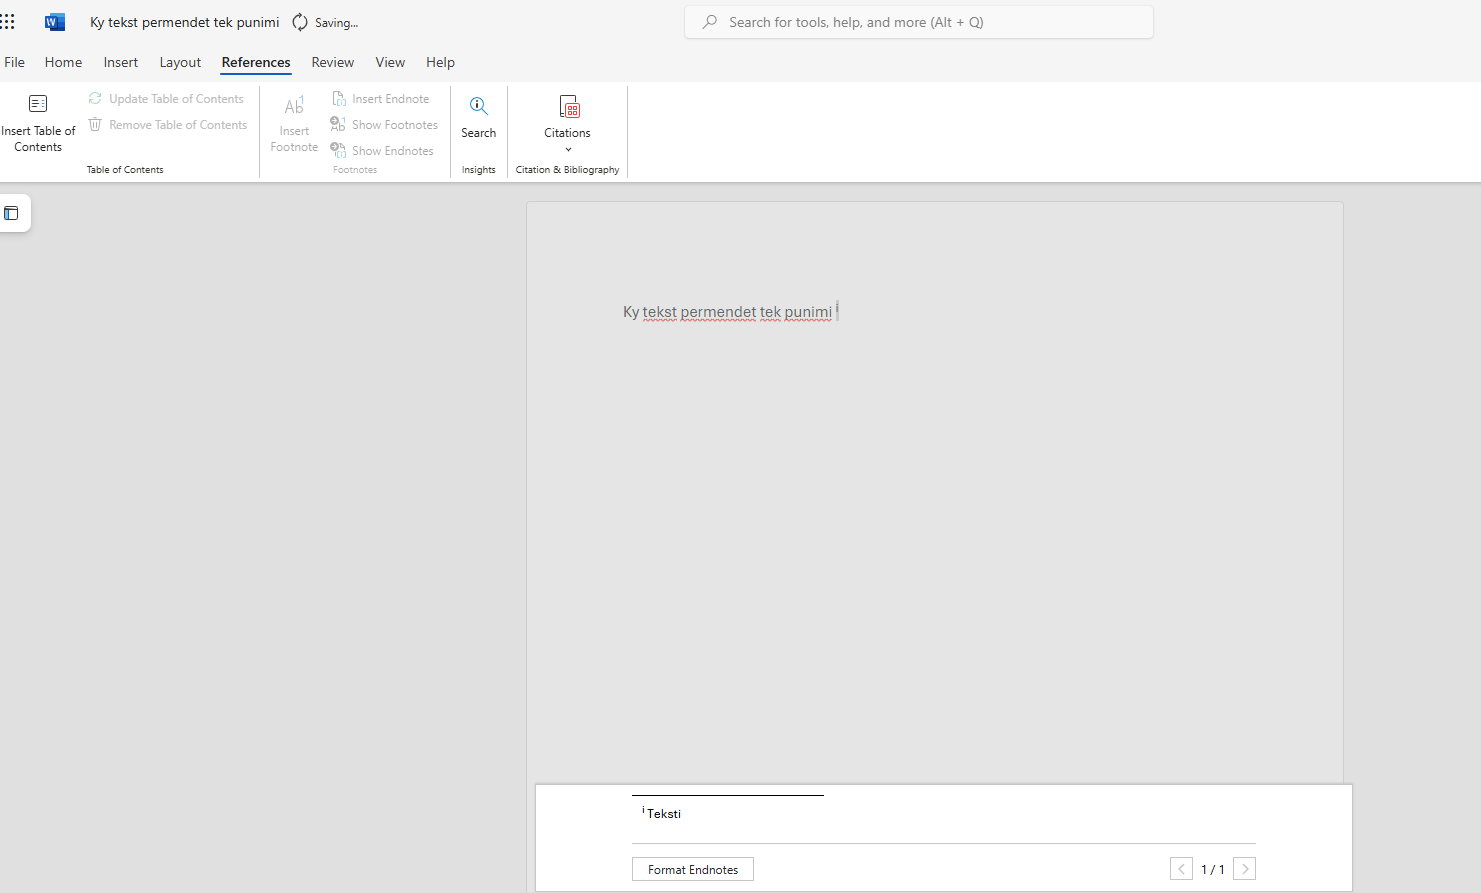
\includegraphics{./images/word14.png}
\end{frame}

\begin{frame}{Redaktimi i një Footnote}
\phantomsection\label{redaktimi-i-njuxeb-footnote}
\begin{enumerate}
\item
  Për të redaktuar një \textbf{footnote}:

  \begin{itemize}
  \item
    Klikoni mbi numrin e \textbf{footnote} në tekstin tuaj.
  \item
    Kaloni automatikisht në fushën e \textbf{footnote} në fund të faqes.
  \end{itemize}
\item
  Bëni ndryshimet e nevojshme në përmbajtjen e shënimit.
\end{enumerate}
\end{frame}

\begin{frame}{Fshirja e një Footnote}
\phantomsection\label{fshirja-e-njuxeb-footnote}
\begin{enumerate}
\item
  Për të \textbf{fshirë} një footnote:

  \begin{itemize}
  \tightlist
  \item
    Shkoni në tekst dhe fshini numrin ose referencën e footnote.
  \end{itemize}
\item
  Shënimi në fund të faqes do të fshihet automatikisht.
\end{enumerate}
\end{frame}

\begin{frame}{Riformatimi i Footnotes}
\phantomsection\label{riformatimi-i-footnotes}
\begin{enumerate}
\item
  Për të ndryshuar stilin e \textbf{footnotes}:

  \begin{itemize}
  \item
    Zgjidhni numrin e footnote ose përmbajtjen.
  \item
    Përdorni opsionet e formatimit nga menyja \textbf{Home} (p.sh.,
    font, madhësi, ngjyrë).
  \end{itemize}
\end{enumerate}
\end{frame}

\begin{frame}{Riformatimi i Footnotes}
\phantomsection\label{riformatimi-i-footnotes-1}
\begin{enumerate}
\setcounter{enumi}{1}
\tightlist
\item
  Formatimi zbatohet vetëm për \textbf{footnote}-n që keni zgjedhur.
\end{enumerate}

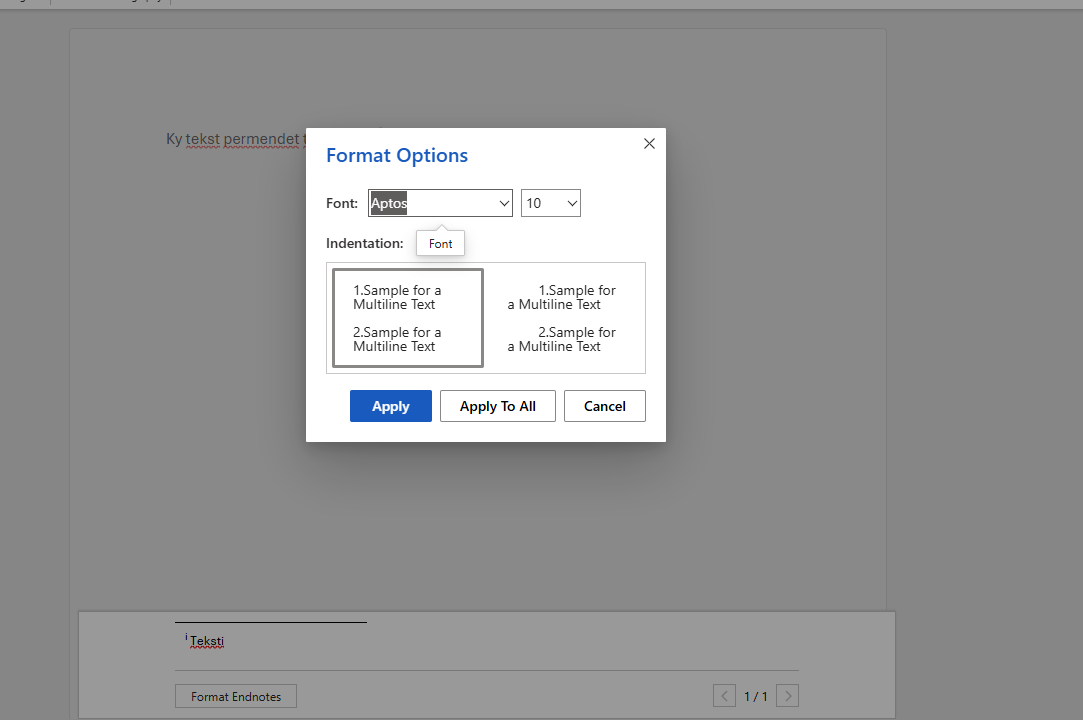
\includegraphics{./images/word15.png}
\end{frame}

\begin{frame}{Përfitimet e përdorimit të Footnotes}
\phantomsection\label{puxebrfitimet-e-puxebrdorimit-tuxeb-footnotes}
\begin{itemize}
\item
  \textbf{Referenca të qarta}: Jepni shpjegime të detajuara pa
  mbingarkuar tekstin kryesor.
\item
  \textbf{Dokumente profesionale}: Ideale për dokumente akademike dhe
  zyrtare.
\item
  \textbf{Organizim më i mirë}: Radhitje dhe numerim automatik i
  footnotes.
\end{itemize}
\end{frame}

\begin{frame}{Rezultate}
\phantomsection\label{rezultate-2}
\begin{itemize}
\item
  \textbf{Footnotes} janë të lehta për t'u futur dhe redaktuar në
  \textbf{Word Web}.
\item
  Ato ndihmojnë në mbajtjen e dokumentit tuaj të pastër dhe të
  organizuar me referenca shtesë.
\item
  Eksploroni funksionet për të riformatuar dhe përmirësuar shënimet
  tuaja.
\end{itemize}
\end{frame}

\begin{frame}{Pyetje \& Diskutim}
\phantomsection\label{pyetje-diskutim-2}
\begin{itemize}
\tightlist
\item
  A keni përdorur më parë \textbf{footnotes} në dokumentet tuaja?
\end{itemize}
\end{frame}

\begin{frame}{Si të futni dhe redaktoni Headers dhe Footers në Word Web}
\phantomsection\label{si-tuxeb-futni-dhe-redaktoni-headers-dhe-footers-nuxeb-word-web}
\begin{itemize}
\item
  \textbf{Headers} dhe \textbf{footers} janë seksione të dokumentit që
  shfaqen në:

  \begin{itemize}
  \item
    \textbf{Header}: Pjesa e sipërme e çdo faqeje.
  \item
    \textbf{Footer}: Pjesa e poshtme e çdo faqeje.
  \end{itemize}
\end{itemize}
\end{frame}

\begin{frame}{Si të futni dhe redaktoni Headers dhe Footers në Word Web}
\phantomsection\label{si-tuxeb-futni-dhe-redaktoni-headers-dhe-footers-nuxeb-word-web-1}
\begin{itemize}
\item
  Ato përdoren për të shtuar:

  \begin{itemize}
  \item
    Tituj të dokumentit.
  \item
    Numra faqesh.
  \item
    Data, emra ose referenca të tjera.
  \end{itemize}
\end{itemize}
\end{frame}

\begin{frame}{Futja e një Header ose Footer}
\phantomsection\label{futja-e-njuxeb-header-ose-footer}
\begin{enumerate}
\item
  Klikoni mbi seksionin \textbf{Insert} në Ribbon.
\item
  Zgjidhni:

  \begin{itemize}
  \item
    \textbf{Header} për të shtuar përmbajtje në krye të faqes.
  \item
    \textbf{Footer} për të shtuar përmbajtje në fund të faqes.
  \end{itemize}
\end{enumerate}
\end{frame}

\begin{frame}{Futja e një Header ose Footer}
\phantomsection\label{futja-e-njuxeb-header-ose-footer-1}
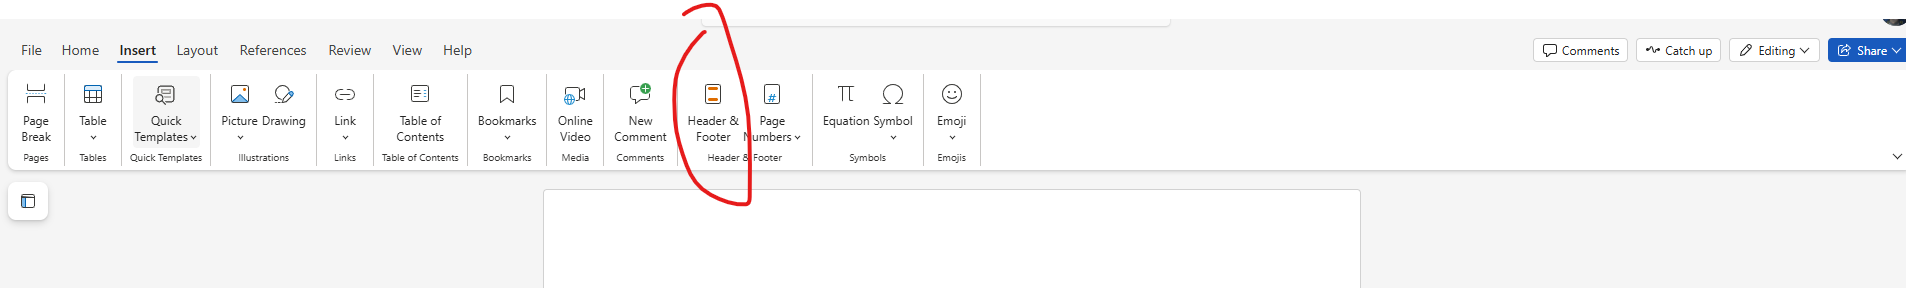
\includegraphics{./images/word16.png}
\end{frame}

\begin{frame}{Futja e një Header ose Footer}
\phantomsection\label{futja-e-njuxeb-header-ose-footer-2}
\begin{enumerate}
\setcounter{enumi}{2}
\item
  Zgjidhni një \textbf{stil të paracaktuar} ose krijoni një bosh.
\item
  Shkruani përmbajtjen tuaj (p.sh., titullin, numrin e faqes, ose
  datën).
\end{enumerate}
\end{frame}

\begin{frame}{Futja e një Header ose Footer}
\phantomsection\label{futja-e-njuxeb-header-ose-footer-3}
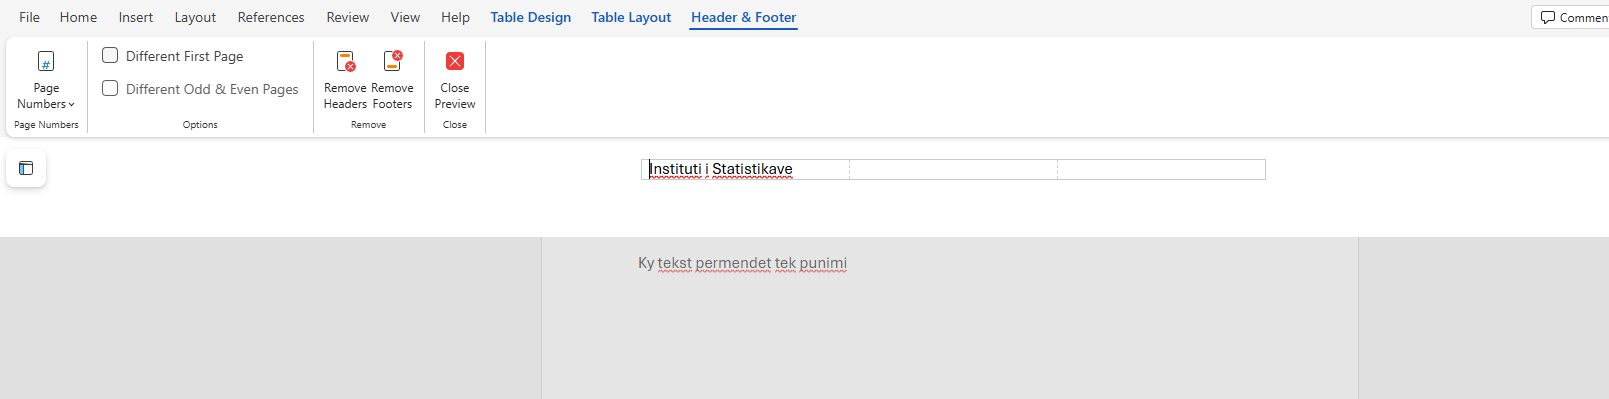
\includegraphics{./images/word17.png}
\end{frame}

\begin{frame}{Redaktimi i Header dhe Footer}
\phantomsection\label{redaktimi-i-header-dhe-footer}
\begin{enumerate}
\item
  Dyfish klikoni mbi zonën \textbf{Header} ose \textbf{Footer} për ta
  aktivizuar atë.
\item
  Për të bërë ndryshime:

  \begin{itemize}
  \item
    Shtoni tekst të ri, data, ose numra faqesh.
  \item
    Përdorni opsionet e formatimit nga menyja \textbf{Home} (font,
    madhësi, ngjyrë).
  \end{itemize}
\item
  Pasi të përfundoni, klikoni \textbf{``Close Header and Footer''} në
  Ribbon.
\end{enumerate}
\end{frame}

\begin{frame}{Shtimi i numrave të faqes në Footer}
\phantomsection\label{shtimi-i-numrave-tuxeb-faqes-nuxeb-footer}
\begin{enumerate}
\item
  Dyfish klikoni në \textbf{Footer} për ta aktivizuar.
\item
  Nga menyja \textbf{Header \& Footer}, klikoni mbi \textbf{Page
  Numbers} (Numra Faqesh).
\end{enumerate}

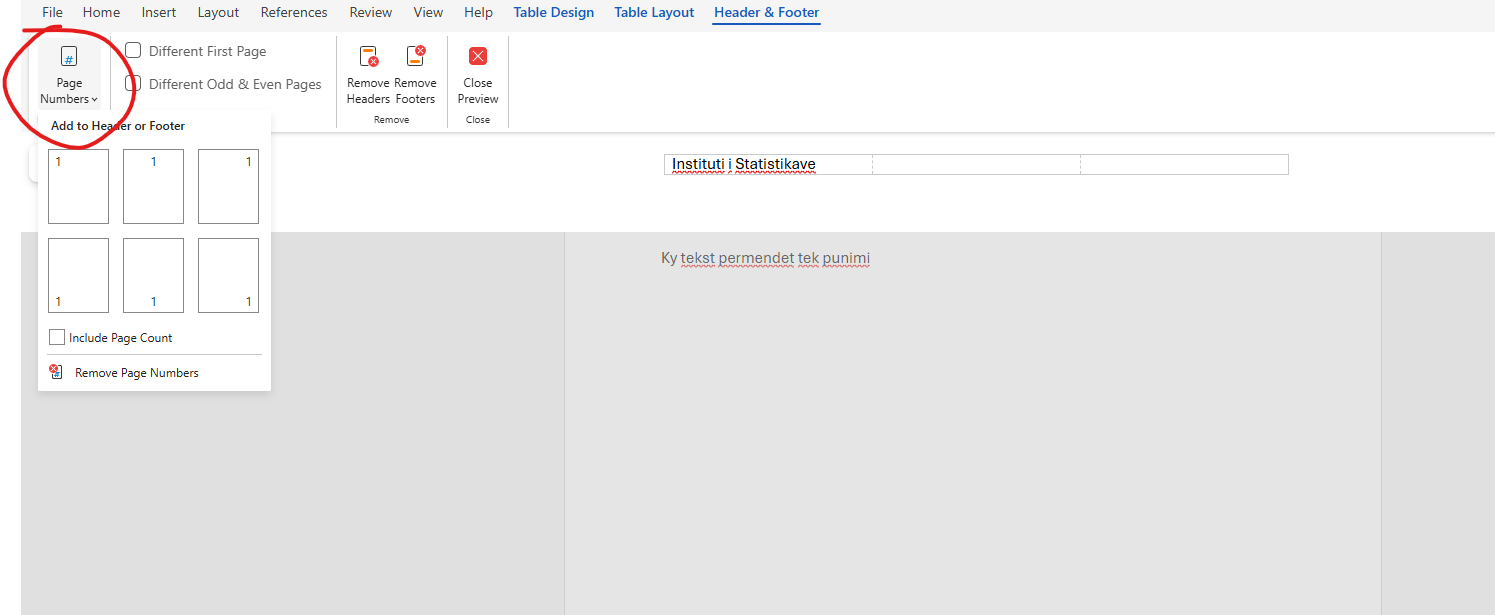
\includegraphics{./images/word18.png}
\end{frame}

\begin{frame}{Shtimi i numrave të faqes në Footer}
\phantomsection\label{shtimi-i-numrave-tuxeb-faqes-nuxeb-footer-1}
\begin{enumerate}
\setcounter{enumi}{2}
\item
  Zgjidhni vendndodhjen e numrit të faqes:

  \begin{itemize}
  \item
    \textbf{Top of Page} (Header)
  \item
    \textbf{Bottom of Page} (Footer)
  \end{itemize}
\item
  Klikoni \textbf{Close Header and Footer} për të ruajtur ndryshimet.
\end{enumerate}
\end{frame}

\begin{frame}{Fshirja e Header ose Footer}
\phantomsection\label{fshirja-e-header-ose-footer}
\begin{enumerate}
\item
  Dyfish klikoni mbi \textbf{Header} ose \textbf{Footer} për ta
  aktivizuar.
\item
  Fshini përmbajtjen manualisht ose përdorni butonin \textbf{Delete}.
\item
  Klikoni \textbf{Close Header and Footer} për të dalë nga zona e
  redaktimit.
\end{enumerate}
\end{frame}

\begin{frame}{Këshilla për përdorimin e Headers dhe Footers}
\phantomsection\label{kuxebshilla-puxebr-puxebrdorimin-e-headers-dhe-footers}
\begin{itemize}
\item
  \textbf{Numërimi i faqes}: Përdorni funksionin \textbf{Page Numbers}
  për të numëruar faqet automatikisht.
\item
  \textbf{Konsistencë}: Përdorni të njëjtin stil në Header dhe Footer
  për një pamje profesionale.
\item
  \textbf{Data dhe tituj}: Shtoni titullin e dokumentit ose datën për
  lehtësinë e referencës.
\end{itemize}
\end{frame}

\begin{frame}{Përfitimet e përdorimit të Headers dhe Footers}
\phantomsection\label{puxebrfitimet-e-puxebrdorimit-tuxeb-headers-dhe-footers}
\begin{itemize}
\item
  \textbf{Organizim më i mirë}: Përmbajtja është e strukturuar dhe më e
  qartë.
\item
  \textbf{Dokumente profesionale}: Përdorim i standardizuar për raportet
  dhe prezantimet.
\item
  \textbf{Navigim i thjeshtë}: Numrat e faqeve ndihmojnë për gjetjen e
  informacionit të saktë.
\end{itemize}
\end{frame}

\begin{frame}{Rezultate}
\phantomsection\label{rezultate-3}
\begin{itemize}
\tightlist
\item
  Futja dhe redaktimi i \textbf{Headers} dhe \textbf{Footers} në Word
  Web është e lehtë dhe ndihmon për të krijuar dokumente të rregullta
  dhe profesionale.\\
\item
  Eksploroni opsionet për të përfshirë numra faqe, tituj dhe të dhëna të
  tjera të rëndësishme.
\end{itemize}
\end{frame}

\begin{frame}{Pyetje \& Diskutim}
\phantomsection\label{pyetje-diskutim-3}
\begin{itemize}
\tightlist
\item
  Cilat elemente përdorni më shpesh në \textbf{Headers} dhe
  \textbf{Footers}?
\end{itemize}
\end{frame}

\begin{frame}{Përmirësimi i Aksesueshmërisë}
\phantomsection\label{puxebrmiruxebsimi-i-aksesueshmuxebrisuxeb}
\begin{enumerate}
\item
  Shkoni te \textbf{Review \textgreater{} Check Accessibility} për të
  bërë dokumentin më të lexueshëm për të gjithë.
\item
  Word do të sugjerojë përmirësime për:

  \begin{itemize}
  \item
    Etiketat e figurave.
  \item
    Kontrastin e ngjyrave.
  \end{itemize}
\end{enumerate}
\end{frame}

\begin{frame}{Përmirësimi i Aksesueshmërisë}
\phantomsection\label{puxebrmiruxebsimi-i-aksesueshmuxebrisuxeb-1}
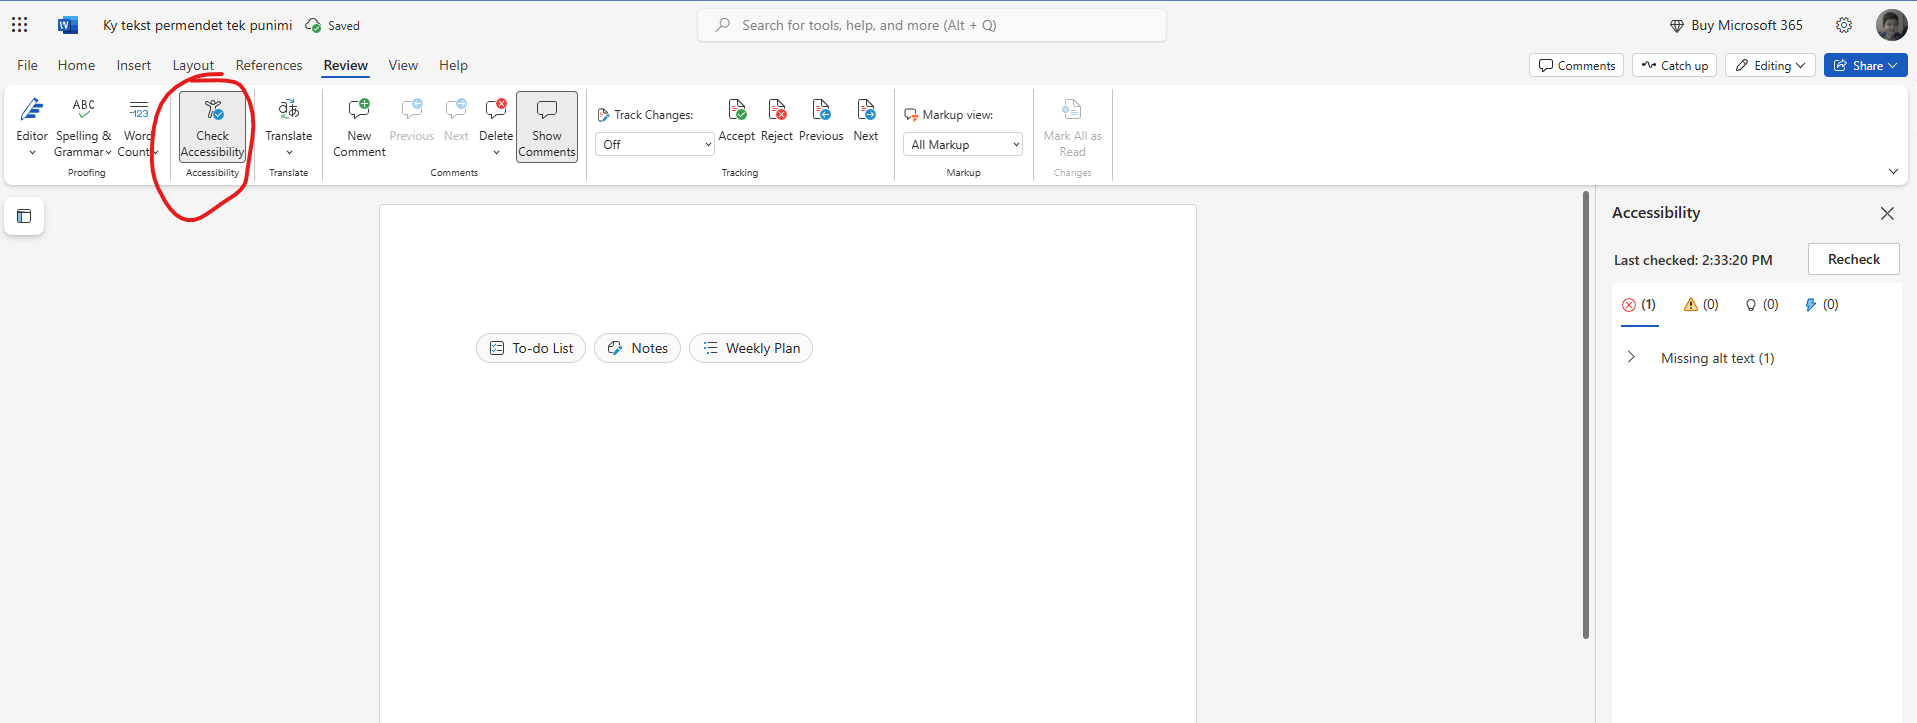
\includegraphics{./images/word26.png}
\end{frame}

\begin{frame}{Rezultate}
\phantomsection\label{rezultate-4}
\begin{itemize}
\item
  Microsoft Word Web ofron mjetet më të rëndësishme për krijimin dhe
  redaktimin e dokumenteve në mënyrë \textbf{të shpejtë dhe të
  thjeshtë}.
\item
  Funksionalitetet si \textbf{Insert}, \textbf{Format}, \textbf{Find \&
  Replace}, dhe \textbf{Share} ju lejojnë të përgatitni dokumente
  profesionale nga çdo pajisje.
\end{itemize}
\end{frame}

\begin{frame}{Pyetje \& Diskutim}
\phantomsection\label{pyetje-diskutim-4}
\begin{itemize}
\tightlist
\item
  Cilat funksione të Word Web përdorni më shpesh?
\end{itemize}
\end{frame}

\section{Microsoft 365 Excel Web}\label{microsoft-365-excel-web}

\begin{frame}{Microsoft 365 Excel Web}
\phantomsection\label{microsoft-365-excel-web-1}
\begin{itemize}
\item
  \textbf{Microsoft Excel Web} është një version online i Excel-it që ju
  lejon:

  \begin{itemize}
  \item
    Të krijoni dhe menaxhoni \textbf{workbooks} nga një shfletues.
  \item
    Të përdorni \textbf{formulat}, \textbf{funksionet}, dhe
    \textbf{tabelat} për analiza të dhënash.
  \item
    Të bashkëpunoni në kohë reale me të tjerët.
  \end{itemize}
\end{itemize}
\end{frame}

\begin{frame}{Microsoft 365 Excel Web}
\phantomsection\label{microsoft-365-excel-web-2}
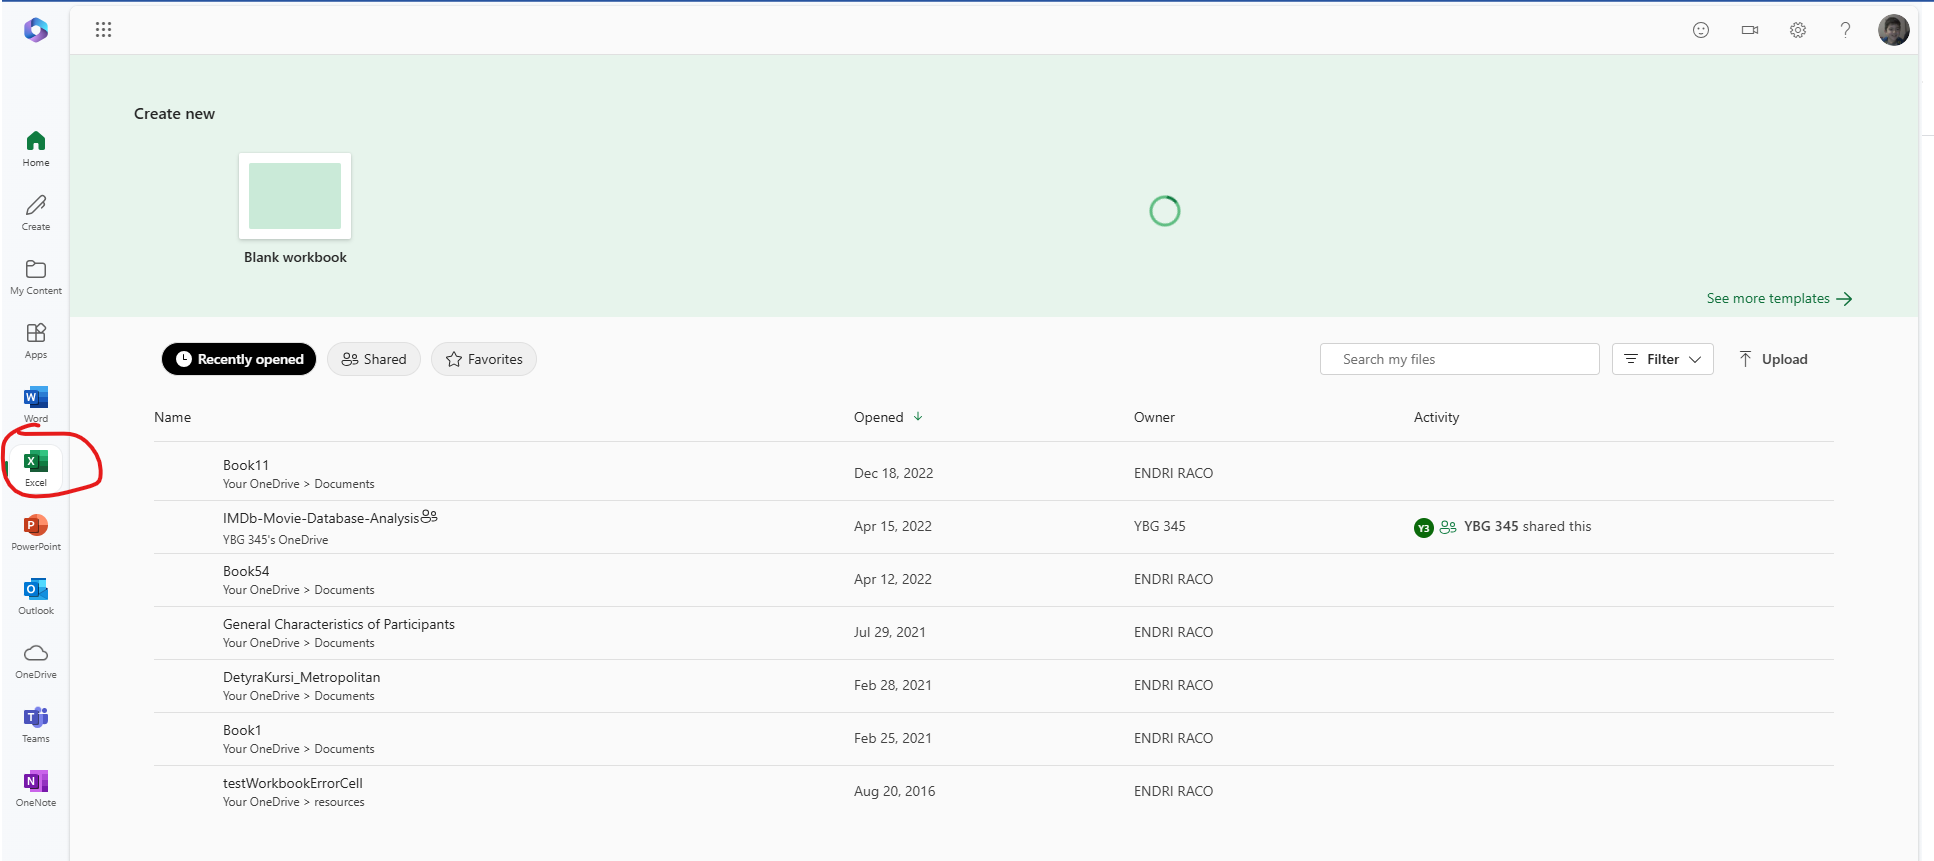
\includegraphics{./images/excel1.png}
\end{frame}

\begin{frame}{Çfarë është Excel?}
\phantomsection\label{uxe7faruxeb-uxebshtuxeb-excel}
\begin{itemize}
\item
  \textbf{Excel} është një mjet për:

  \begin{itemize}
  \item
    Organizimin dhe analizën e të dhënave.
  \item
    Kryerjen e llogaritjeve duke përdorur \textbf{formulat} dhe
    \textbf{funksionet}.
  \item
    Vizualizimin e të dhënave përmes \textbf{grafikëve dhe tabelave}.
  \end{itemize}
\end{itemize}
\end{frame}

\begin{frame}{Krijimi i një Workbook të Ri}
\phantomsection\label{krijimi-i-njuxeb-workbook-tuxeb-ri}
\begin{enumerate}
\item
  Hapni shfletuesin dhe shkoni te:\\
  \textbf{\url{https://www.office.com}}.
\item
  Identifikohuni me kredencialet tuaja të \textbf{Microsoft 365}.
\item
  Klikoni mbi \textbf{Excel} \textgreater{} \textbf{New Blank Workbook}.
\end{enumerate}
\end{frame}

\begin{frame}{Krijimi i një Workbook të Ri}
\phantomsection\label{krijimi-i-njuxeb-workbook-tuxeb-ri-1}
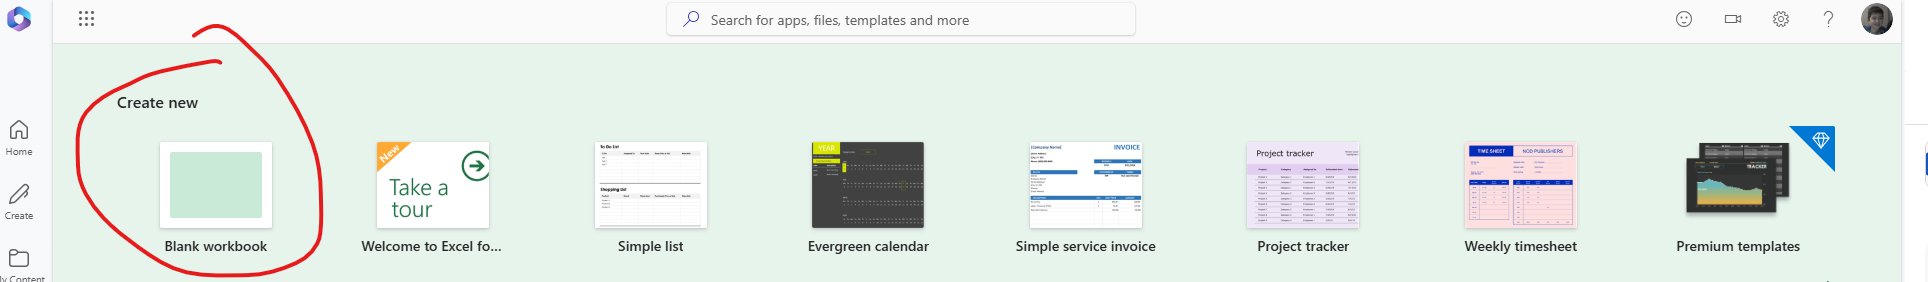
\includegraphics{./images/excel2.png}
\end{frame}

\begin{frame}{Futja dhe Fshirja e Fletëve (Worksheets)}
\phantomsection\label{futja-dhe-fshirja-e-fletuxebve-worksheets}
\begin{enumerate}
\item
  Për të \textbf{shtuar një fletë}:

  \begin{itemize}
  \tightlist
  \item
    Klikoni mbi \textbf{+} pranë emrave të fletëve në fund të ekranit.
  \end{itemize}
\end{enumerate}
\end{frame}

\begin{frame}{Futja dhe Fshirja e Fletëve (Worksheets)}
\phantomsection\label{futja-dhe-fshirja-e-fletuxebve-worksheets-1}
\begin{enumerate}
\setcounter{enumi}{1}
\item
  Për të \textbf{fshirë një fletë}:

  \begin{itemize}
  \tightlist
  \item
    Klikoni me të djathtën mbi emrin e fletës \textgreater{}
    \textbf{Delete}.
  \end{itemize}
\end{enumerate}
\end{frame}

\begin{frame}{Futja dhe Fshirja e Fletëve (Worksheets)}
\phantomsection\label{futja-dhe-fshirja-e-fletuxebve-worksheets-2}
\begin{enumerate}
\setcounter{enumi}{2}
\item
  Për të \textbf{kopjuar} ose \textbf{lëvizur} një fletë:

  \begin{itemize}
  \tightlist
  \item
    Klikoni me të djathtën \textgreater{} \textbf{Move or Copy}.
  \end{itemize}
\end{enumerate}
\end{frame}

\begin{frame}{Futja dhe Fshirja e Fletëve (Worksheets)}
\phantomsection\label{futja-dhe-fshirja-e-fletuxebve-worksheets-3}
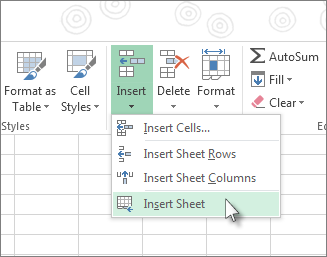
\includegraphics{./images/excel3.png}
\end{frame}

\begin{frame}{Menaxhimi i Rreshtave dhe Kolonave}
\phantomsection\label{menaxhimi-i-rreshtave-dhe-kolonave}
\begin{itemize}
\item
  Në \textbf{Microsoft Excel Web}, mund të:

  \begin{itemize}
  \item
    Shtoni ose fshini \textbf{rreshta} dhe \textbf{kolona}.
  \item
    Bllokoni (freeze) rreshtat ose kolonat për referencë të lehtë.
  \item
    Filtroni dhe pastroni të dhënat për \textbf{vlera unike} dhe
    \textbf{duplikate}.
  \item
    Shpërndani të dhënat duke përdorur \textbf{Text to Columns}.
  \end{itemize}
\end{itemize}
\end{frame}

\begin{frame}{Futja ose Fshirja e Rreshtave dhe Kolonave}
\phantomsection\label{futja-ose-fshirja-e-rreshtave-dhe-kolonave}
\begin{enumerate}
\item
  Klikoni me të djathtën mbi numrin e \textbf{rreshtit} ose shkronjën e
  \textbf{kolonës}.
\item
  Zgjidhni \textbf{Insert} për të futur një rresht/kolonë të ri.
\end{enumerate}
\end{frame}

\begin{frame}{Futja ose Fshirja e Rreshtave dhe Kolonave}
\phantomsection\label{futja-ose-fshirja-e-rreshtave-dhe-kolonave-1}
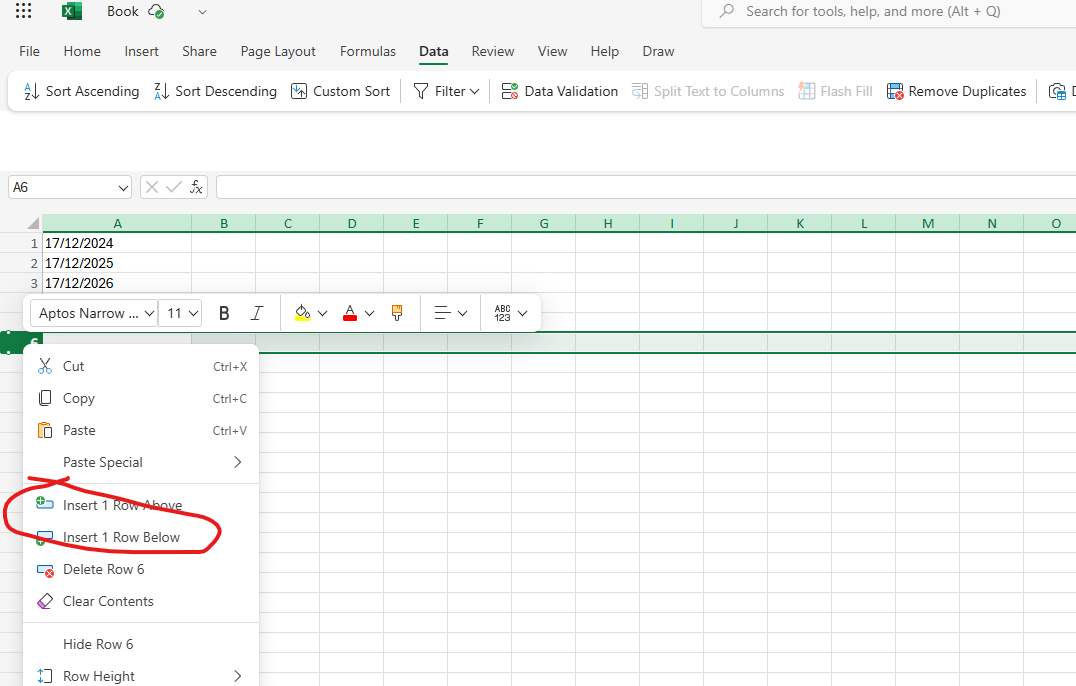
\includegraphics{./images/excel4.png}
\end{frame}

\begin{frame}{Fshirja e Rreshtave/Kolonave}
\phantomsection\label{fshirja-e-rreshtavekolonave}
\begin{enumerate}
\item
  Klikoni me të djathtën mbi rreshtin/kolonën që dëshironi të fshini.
\item
  Zgjidhni \textbf{Delete} për ta hequr atë.
\end{enumerate}
\end{frame}

\begin{frame}{Fshirja e Rreshtave/Kolonave}
\phantomsection\label{fshirja-e-rreshtavekolonave-1}
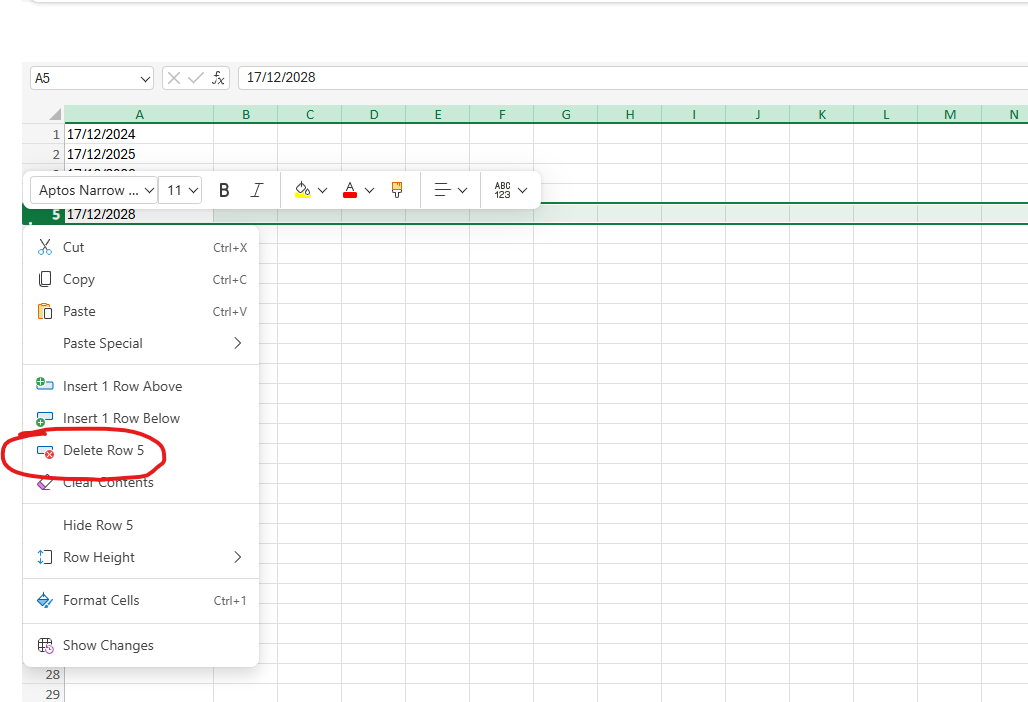
\includegraphics{./images/excel5.png}
\end{frame}

\begin{frame}{Zgjedhja e Përmbajtjes së Qelizave}
\phantomsection\label{zgjedhja-e-puxebrmbajtjes-suxeb-qelizave}
\begin{enumerate}
\tightlist
\item
  Klikoni dhe tërhiqni për të zgjedhur një gamë të qelizave.
\end{enumerate}
\end{frame}

\begin{frame}{Zgjedhja e Përmbajtjes së Qelizave}
\phantomsection\label{zgjedhja-e-puxebrmbajtjes-suxeb-qelizave-1}
\begin{enumerate}
\setcounter{enumi}{1}
\item
  Për të zgjedhur të gjithë rreshtin ose kolonën:

  \begin{itemize}
  \tightlist
  \item
    Klikoni numrin e \textbf{rreshtit} (majtas) ose shkronjën e
    \textbf{kolonës} (sipër).
  \end{itemize}
\end{enumerate}

\textbf{Shkurt}:

\begin{itemize}
\tightlist
\item
  \textbf{Ctrl + A}: Zgjedh të gjithë përmbajtjen e worksheet-it.
\end{itemize}
\end{frame}

\begin{frame}{Ngrirja e Rreshtave dhe Kolonave (Freeze Panes)}
\phantomsection\label{ngrirja-e-rreshtave-dhe-kolonave-freeze-panes}
\begin{enumerate}
\tightlist
\item
  Shkoni te menyja \textbf{View} në Ribbon.
\end{enumerate}
\end{frame}

\begin{frame}{Ngrirja e Rreshtave dhe Kolonave (Freeze Panes)}
\phantomsection\label{ngrirja-e-rreshtave-dhe-kolonave-freeze-panes-1}
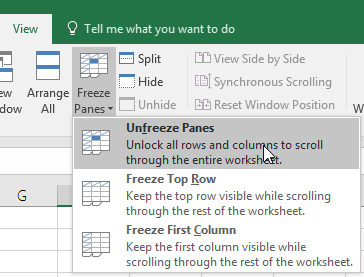
\includegraphics{./images/excel7.png}
\end{frame}

\begin{frame}{Ngrirja e Rreshtave dhe Kolonave (Freeze Panes)}
\phantomsection\label{ngrirja-e-rreshtave-dhe-kolonave-freeze-panes-2}
\begin{enumerate}
\setcounter{enumi}{1}
\item
  Zgjidhni \textbf{Freeze Panes} për të bllokuar:

  \begin{itemize}
  \item
    \textbf{Freeze Top Row}: Ngrin vetëm rreshtin e parë.
  \item
    \textbf{Freeze First Column}: Ngrin vetëm kolonën e parë.
  \end{itemize}
\end{enumerate}

\textbf{Përdorimi}: Ky funksion është i dobishëm për të mbajtur titujt e
tabelës gjithmonë të dukshëm.
\end{frame}

\begin{frame}{Fshehja ose Shfaqja e Rreshtave/Kolonave}
\phantomsection\label{fshehja-ose-shfaqja-e-rreshtavekolonave}
\begin{enumerate}
\item
  Klikoni me të djathtën mbi numrin e \textbf{rreshtit} ose shkronjën e
  \textbf{kolonës}.
\item
  Zgjidhni \textbf{Hide} (Fshihe).
\end{enumerate}
\end{frame}

\begin{frame}{Shfaqja e Rreshtave/Kolonave}
\phantomsection\label{shfaqja-e-rreshtavekolonave}
\begin{enumerate}
\item
  Zgjidhni rreshtat ose kolonat që ndodhen para dhe pas zonës së
  fshehur.
\item
  Klikoni me të djathtën dhe zgjidhni \textbf{Unhide} (Shfaq).
\end{enumerate}
\end{frame}

\begin{frame}{Filtrimi për Vlera Unike ose Heqja e Duplikatëve}
\phantomsection\label{filtrimi-puxebr-vlera-unike-ose-heqja-e-duplikatuxebve}
\begin{enumerate}
\item
  Zgjidhni të dhënat që dëshironi të filtroni.
\item
  Shkoni te \textbf{Data \textgreater{} Remove Duplicates} për të hequr
  vlerat e përsëritura.
\item
  Përdorni \textbf{Filter} për të shfaqur vetëm vlerat unike.
\end{enumerate}
\end{frame}

\begin{frame}{Filtrimi për Vlera Unike ose Heqja e Duplikatëve}
\phantomsection\label{filtrimi-puxebr-vlera-unike-ose-heqja-e-duplikatuxebve-1}
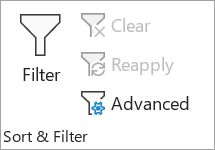
\includegraphics{./images/excel8.png}
\end{frame}

\begin{frame}{Ndarja e Tekstit me Convert Text to Columns}
\phantomsection\label{ndarja-e-tekstit-me-convert-text-to-columns}
\begin{enumerate}
\item
  Zgjidhni kolonën që përmban tekst të bashkuar (p.sh., Emër dhe
  Mbiemër).
\item
  Shkoni te \textbf{Data \textgreater{} Text to Columns}.
\end{enumerate}
\end{frame}

\begin{frame}{Ndarja e Tekstit me Convert Text to Columns}
\phantomsection\label{ndarja-e-tekstit-me-convert-text-to-columns-1}
\begin{enumerate}
\setcounter{enumi}{2}
\item
  Zgjidhni llojin e ndarjes:

  \begin{itemize}
  \tightlist
  \item
    \textbf{Delimited}: Përdorni ndarës si presja, pika ose hapësira.
  \end{itemize}
\item
  Klikoni \textbf{Finish} për të ndarë të dhënat në kolona të veçanta.
\end{enumerate}
\end{frame}

\begin{frame}{Krijimi i Një Liste me Data Sekuenciale}
\phantomsection\label{krijimi-i-njuxeb-liste-me-data-sekuenciale}
\begin{enumerate}
\item
  Klikoni në qelizën ku dëshironi të filloni listën.
\item
  Shkruani datën e parë (p.sh., 01/01/2024).
\end{enumerate}
\end{frame}

\begin{frame}{Krijimi i Një Liste me Data Sekuenciale}
\phantomsection\label{krijimi-i-njuxeb-liste-me-data-sekuenciale-1}
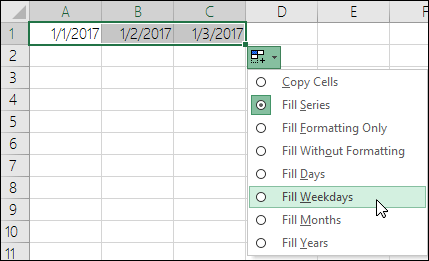
\includegraphics{./images/excel9.png}
\end{frame}

\begin{frame}{Krijimi i Një Liste me Data Sekuenciale}
\phantomsection\label{krijimi-i-njuxeb-liste-me-data-sekuenciale-2}
\begin{enumerate}
\setcounter{enumi}{2}
\item
  Përdorni \textbf{AutoFill handle}:

  \begin{itemize}
  \tightlist
  \item
    Tërhiqni në poshtë ose djathtas për të plotësuar datat.
  \end{itemize}
\item
  Excel do të krijojë automatikisht një listë të datave sekuenciale.
\end{enumerate}
\end{frame}

\begin{frame}{Lëvizja ose Kopjimi i Qelizave dhe Përmbajtjes së Tyre}
\phantomsection\label{luxebvizja-ose-kopjimi-i-qelizave-dhe-puxebrmbajtjes-suxeb-tyre}
\begin{enumerate}
\item
  Zgjidhni qelizat që dëshironi të lëvizni.
\item
  Vendosni kursorin në kufirin e qelizave të zgjedhura.
\item
  Tërhiqni qelizat në vendin e ri.
\end{enumerate}
\end{frame}

\begin{frame}{Kopjimi i Qelizave:}
\phantomsection\label{kopjimi-i-qelizave}
\begin{enumerate}
\item
  Zgjidhni qelizat.
\item
  Klikoni \textbf{Ctrl + C} për të kopjuar.
\item
  Vendosni kursorin në destinacion dhe shtypni \textbf{Ctrl + V} për të
  ngjitur (paste).
\end{enumerate}
\end{frame}

\begin{frame}{Kopjimi i Qelizave:}
\phantomsection\label{kopjimi-i-qelizave-1}
\textbf{Shkurt}:

\begin{itemize}
\tightlist
\item
  \textbf{Ctrl + X}: Prerje (Cut).\\
\item
  \textbf{Ctrl + C}: Kopjim (Copy).\\
\item
  \textbf{Ctrl + V}: Ngjitje (Paste).
\end{itemize}
\end{frame}

\begin{frame}{Ndryshimi i Gjerësisë së Kolonave ose Lartësisë së
Rreshtave}
\phantomsection\label{ndryshimi-i-gjeruxebsisuxeb-suxeb-kolonave-ose-lartuxebsisuxeb-suxeb-rreshtave}
\begin{enumerate}
\item
  Vendosni kursorin mbi ndarësin midis dy shkronjave të kolonave (p.sh.,
  A dhe B).
\item
  Tërhiqni për të zgjeruar ose ngushtuar kolonën.
\end{enumerate}
\end{frame}

\begin{frame}{Për të ndryshuar lartësinë e rreshtave:}
\phantomsection\label{puxebr-tuxeb-ndryshuar-lartuxebsinuxeb-e-rreshtave}
\begin{enumerate}
\item
  Vendosni kursorin mbi ndarësin midis numrave të rreshtave (p.sh., 1
  dhe 2).
\item
  Tërhiqni për të ndryshuar madhësinë.
\end{enumerate}
\end{frame}

\begin{frame}{Gjetja dhe Zëvendësimi i Tekstit dhe Numrave}
\phantomsection\label{gjetja-dhe-zuxebvenduxebsimi-i-tekstit-dhe-numrave}
\begin{enumerate}
\item
  Shkoni te \textbf{Home \textgreater{} Find \& Select}.
\item
  Zgjidhni \textbf{Find} për të kërkuar tekst ose numra në worksheet.
\end{enumerate}

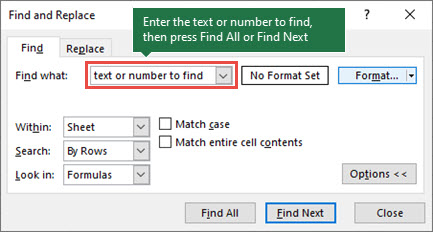
\includegraphics{./images/excel10.jpg}
\end{frame}

\begin{frame}{Gjetja dhe Zëvendësimi i Tekstit dhe Numrave}
\phantomsection\label{gjetja-dhe-zuxebvenduxebsimi-i-tekstit-dhe-numrave-1}
\begin{enumerate}
\setcounter{enumi}{2}
\item
  Për të zëvendësuar:

  \begin{itemize}
  \item
    Zgjidhni \textbf{Replace}.
  \item
    Vendosni tekstin që kërkoni dhe tekstin zëvendësues.
  \item
    Klikoni \textbf{Replace All} për të zëvendësuar të gjitha rastet.
  \end{itemize}
\end{enumerate}
\end{frame}

\begin{frame}{Bashkimi dhe Ndarja e Qelizave (Merge/Unmerge)}
\phantomsection\label{bashkimi-dhe-ndarja-e-qelizave-mergeunmerge}
\begin{enumerate}
\item
  Zgjidhni qelizat që dëshironi të bashkoni.
\item
  Shkoni te \textbf{Home \textgreater{} Merge \& Center}.
\end{enumerate}
\end{frame}

\begin{frame}{Bashkimi dhe Ndarja e Qelizave (Merge/Unmerge)}
\phantomsection\label{bashkimi-dhe-ndarja-e-qelizave-mergeunmerge-1}
\begin{enumerate}
\setcounter{enumi}{2}
\item
  Zgjidhni një opsion:

  \begin{itemize}
  \item
    \textbf{Merge \& Center}: Bashkon qelizat dhe qendra tekstin.
  \item
    \textbf{Merge Across}: Bashkon qelizat në të njëjtën rresht.
  \item
    \textbf{Merge Cells}: Bashkon qelizat pa qendruar tekstin.
  \end{itemize}
\end{enumerate}
\end{frame}

\begin{frame}{Ndarja e Qelizave:}
\phantomsection\label{ndarja-e-qelizave}
\begin{enumerate}
\item
  Zgjidhni një qelizë të bashkuar.
\item
  Shkoni te \textbf{Home \textgreater{} Merge \& Center} dhe zgjidhni
  \textbf{Unmerge Cells}.
\end{enumerate}
\end{frame}

\begin{frame}{Aplikimi i Data Validation për Qelizat}
\phantomsection\label{aplikimi-i-data-validation-puxebr-qelizat}
\begin{enumerate}
\item
  Zgjidhni qelizat ku dëshironi të aplikoni \textbf{Data Validation}.
\item
  Shkoni te \textbf{Data \textgreater{} Data Validation}.
\end{enumerate}

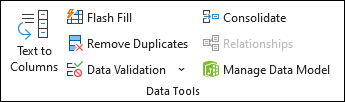
\includegraphics{./images/excel11.png}
\end{frame}

\begin{frame}{Aplikimi i Data Validation për Qelizat}
\phantomsection\label{aplikimi-i-data-validation-puxebr-qelizat-1}
\begin{enumerate}
\setcounter{enumi}{2}
\item
  Zgjidhni kriteret:

  \begin{itemize}
  \item
    \textbf{List}: Vendosni një listë me vlera të lejuara.
  \item
    \textbf{Whole number}: Lejon vetëm numra të plotë.
  \item
    \textbf{Date}: Lejon vetëm data të vlefshme.
  \end{itemize}
\end{enumerate}
\end{frame}

\begin{frame}{Aplikimi i Data Validation për Qelizat}
\phantomsection\label{aplikimi-i-data-validation-puxebr-qelizat-2}
\begin{enumerate}
\setcounter{enumi}{3}
\tightlist
\item
  Klikoni \textbf{OK} për të ruajtur ndryshimet.
\end{enumerate}
\end{frame}

\begin{frame}{Importimi dhe Eksportimi i Skedarëve .txt ose .csv}
\phantomsection\label{importimi-dhe-eksportimi-i-skedaruxebve-.txt-ose-.csv}
\begin{block}{Importimi i Skedarëve .txt/.csv:}
\phantomsection\label{importimi-i-skedaruxebve-.txt.csv}
\begin{enumerate}
\item
  Shkoni te \textbf{File \textgreater{} Open}.
\item
  Ngarkoni skedarin \textbf{.csv} ose \textbf{.txt}.
\item
  Excel do të konvertojë automatikisht të dhënat dhe t'i paraqesë ato në
  worksheet.
\end{enumerate}
\end{block}
\end{frame}

\begin{frame}{Eksportimi i Skedarëve .csv:}
\phantomsection\label{eksportimi-i-skedaruxebve-.csv}
\begin{enumerate}
\item
  Shkoni te \textbf{File \textgreater{} Save As}.
\item
  Zgjidhni \textbf{.csv} si formatin e ruajtjes.
\item
  Klikoni \textbf{Download} për të shkarkuar skedarin.
\end{enumerate}
\end{frame}

\begin{frame}{Formatet Numerike të Disponueshme}
\phantomsection\label{formatet-numerike-tuxeb-disponueshme}
\begin{enumerate}
\item
  Zgjidhni qelizat me të dhëna numerike.
\item
  Shkoni te \textbf{Home \textgreater{} Number Format}.
\end{enumerate}
\end{frame}

\begin{frame}{Formatet Numerike të Disponueshme}
\phantomsection\label{formatet-numerike-tuxeb-disponueshme-1}
\begin{enumerate}
\setcounter{enumi}{2}
\item
  Zgjidhni një format nga lista:

  \begin{itemize}
  \item
    \textbf{General}: Format i paracaktuar.
  \item
    \textbf{Number}: Numra me presje dhe decimale.
  \item
    \textbf{Currency}: Monedha (p.sh., €, \$, £).
  \item
    \textbf{Date}: Formate të ndryshme të datës.
  \item
    \textbf{Percentage}: Shndërron numrat në përqindje.
  \item
    \textbf{Text}: Trajton numrat si tekst.
  \end{itemize}
\end{enumerate}
\end{frame}

\begin{frame}{Conditional Formatting (Formatimi Kushtor)}
\phantomsection\label{conditional-formatting-formatimi-kushtor}
\begin{enumerate}
\item
  Zgjidhni qelizat që dëshironi të formatoni.
\item
  Shkoni te \textbf{Home \textgreater{} Conditional Formatting}.
\end{enumerate}
\end{frame}

\begin{frame}{Conditional Formatting (Formatimi Kushtor)}
\phantomsection\label{conditional-formatting-formatimi-kushtor-1}
\begin{enumerate}
\setcounter{enumi}{2}
\item
  Zgjidhni një rregull të formatimit:

  \begin{itemize}
  \item
    \textbf{Highlight Cells Rules}: Formatoni qelizat që përmbajnë vlera
    specifike.
  \item
    \textbf{Top/Bottom Rules}: Formatoni vlerat më të larta/më të ulëta.
  \item
    \textbf{Color Scales}: Aplikoni një gradient me ngjyra.
  \end{itemize}
\end{enumerate}
\end{frame}

\begin{frame}{Conditional Formatting (Formatimi Kushtor)}
\phantomsection\label{conditional-formatting-formatimi-kushtor-2}
\begin{enumerate}
\setcounter{enumi}{3}
\tightlist
\item
  Klikoni \textbf{OK} për të aplikuar rregullin.
\end{enumerate}

\textbf{Shembull}: Formatoni qelizat me vlera \textgreater{} 100 me
ngjyrë të verdhë.
\end{frame}

\begin{frame}{Shtrirja dhe Rrotullimi i Tekstit}
\phantomsection\label{shtrirja-dhe-rrotullimi-i-tekstit}
\begin{enumerate}
\item
  Zgjidhni qelizën ose qelizat që përmbajnë tekst.
\item
  Shkoni te \textbf{Home \textgreater{} Orientation}.
\end{enumerate}

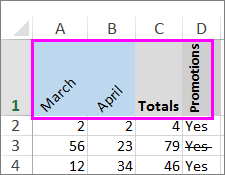
\includegraphics{./images/excel12.png}
\end{frame}

\begin{frame}{Shtrirja dhe Rrotullimi i Tekstit}
\phantomsection\label{shtrirja-dhe-rrotullimi-i-tekstit-1}
\begin{enumerate}
\setcounter{enumi}{2}
\item
  Opsionet e disponueshme:

  \begin{itemize}
  \item
    \textbf{Align Left/Center/Right}: Shtrirja horizontale.
  \item
    \textbf{Align Top/Middle/Bottom}: Shtrirja vertikale.
  \item
    \textbf{Orientation}: Rrotulloni tekstin me kënd specifik (p.sh.,
    45°).
  \end{itemize}
\end{enumerate}
\end{frame}

\begin{frame}{Ndryshimi i Formatit të Qelizës}
\phantomsection\label{ndryshimi-i-formatit-tuxeb-qelizuxebs}
\begin{enumerate}
\item
  Zgjidhni qelizën që dëshironi të formatoni.
\item
  Klikoni me të djathtën dhe zgjidhni \textbf{Format Cells}.
\end{enumerate}
\end{frame}

\begin{frame}{Ndryshimi i Formatit të Qelizës}
\phantomsection\label{ndryshimi-i-formatit-tuxeb-qelizuxebs-1}
\begin{enumerate}
\setcounter{enumi}{2}
\item
  Opsionet për ndryshimin e formatit përfshijnë:

  \begin{itemize}
  \item
    \textbf{Font}: Stili, madhësia dhe ngjyra e tekstit.
  \item
    \textbf{Fill}: Ngjyra e sfondit të qelizës.
  \item
    \textbf{Border}: Kufijtë e qelizës.
  \end{itemize}
\end{enumerate}
\end{frame}

\begin{frame}{Kopjimi i Formatit të Qelizave}
\phantomsection\label{kopjimi-i-formatit-tuxeb-qelizave}
\begin{enumerate}
\item
  Zgjidhni qelizën që ka formatin që dëshironi të kopjoni.
\item
  Klikoni mbi \textbf{Format Painter} në Ribbon (Home).
\item
  Klikoni mbi qelizën/qelizat ku dëshironi të aplikoni formatin.
\end{enumerate}
\end{frame}

\begin{frame}{Kopjimi i Formatit të Qelizave}
\phantomsection\label{kopjimi-i-formatit-tuxeb-qelizave-1}
\textbf{Këshillë}: Format Painter mund të përdoret disa herë duke
dyfishtë klikuar mbi të.
\end{frame}

\begin{frame}{Shfaqja ose Fshehja e Vlerave Zero}
\phantomsection\label{shfaqja-ose-fshehja-e-vlerave-zero}
\begin{enumerate}
\item
  Shkoni te \textbf{File \textgreater{} Options} (nëse është e
  disponueshme në Excel Web).
\item
  Alternative, përdorni \textbf{Conditional Formatting} për të bërë
  qelizat me vlerë zero të padukshme:

  \begin{itemize}
  \tightlist
  \item
    Vendosni fontin me ngjyrën e bardhë për vlerat 0.
  \end{itemize}
\end{enumerate}
\end{frame}

\begin{frame}[fragile]{Shfaqja ose Fshehja e Vlerave Zero}
\phantomsection\label{shfaqja-ose-fshehja-e-vlerave-zero-1}
\textbf{Zgjidhje tjetër}: Përdorni një formulë \texttt{IF}:

\begin{Shaded}
\begin{Highlighting}[]
\NormalTok{   =IF(A1=0, "", A1)}
\end{Highlighting}
\end{Shaded}

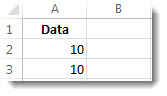
\includegraphics{./images/excel13.jpg}
\end{frame}

\begin{frame}{Formulat dhe Funksionet}
\phantomsection\label{formulat-dhe-funksionet}
\begin{itemize}
\item
  \textbf{Microsoft Excel} ofron formula dhe funksione të fuqishme për
  të kryer analiza të të dhënave.
\item
  Në këtë prezantim do të mbulojmë funksionet kryesore, përfshirë:

  \begin{itemize}
  \item
    \textbf{SUM}, \textbf{COUNTIF}, dhe \textbf{IF}.
  \item
    \textbf{VLOOKUP} dhe \textbf{XLOOKUP} për kërkime.
  \item
    \textbf{SUMIFS} dhe \textbf{MATCH} për raste më komplekse.
  \end{itemize}
\end{itemize}
\end{frame}

\begin{frame}{Pasqyrë e Formulave në Excel}
\phantomsection\label{pasqyruxeb-e-formulave-nuxeb-excel}
\begin{itemize}
\item
  Formulat në Excel fillojnë gjithmonë me një \textbf{=}.
\item
  Struktura bazë:
\end{itemize}

\$ =FUNKSION(argument1, argument2, \ldots) \$
\end{frame}

\begin{frame}{Pasqyrë e Formulave në Excel}
\phantomsection\label{pasqyruxeb-e-formulave-nuxeb-excel-1}
\$ =SUM(A1:A10)\$ mbledh vlerat nga qelizat A1 deri në A10.

\(=IF(B2>50, "Po", "Jo")\) kontrollon nëse vlera në B2 është më e madhe
se 50.
\end{frame}

\begin{frame}[fragile]{Funksioni SUM}
\phantomsection\label{funksioni-sum}
Përdoret për të mbledhur vlera numerike në një gamë qelizash.

Sintaksa:

\begin{Shaded}
\begin{Highlighting}[]
\NormalTok{=SUM(numri1, numri2, ...)}
\end{Highlighting}
\end{Shaded}
\end{frame}

\begin{frame}{Funksioni SUM}
\phantomsection\label{funksioni-sum-1}
\(=SUM(A1:A5)\) mbledh vlerat në qelizat A1 deri A5.

\(=SUM(A1, B1, C1)\) mbledh vlerat individuale.
\end{frame}

\begin{frame}{Funksioni COUNTIF}
\phantomsection\label{funksioni-countif}
Numëron qelizat që plotësojnë një kusht specifik.

Sintaksa:

\$ =COUNTIF(gama, kushti)\$
\end{frame}

\begin{frame}{Funksioni COUNTIF}
\phantomsection\label{funksioni-countif-1}
\(=COUNTIF(A1:A10, ">50")\) numëron qelizat me vlera më të mëdha se 50.
\(=COUNTIF(B1:B20, "Po")\) numëron qelizat që përmbajnë ``Po''.
\end{frame}

\begin{frame}[fragile]{Funksioni IF}
\phantomsection\label{funksioni-if}
Kontrollon nëse një kusht është i vërtetë apo jo dhe kthen rezultate të
ndryshme.

Sintaksa:

\begin{Shaded}
\begin{Highlighting}[]
\NormalTok{=IF(kushti, vlera\_nëse\_vërtetë, vlera\_nëse\_gabuar)}
\end{Highlighting}
\end{Shaded}
\end{frame}

\begin{frame}{Funksioni IF}
\phantomsection\label{funksioni-if-1}
\(=IF(A1>50, "Kaluar", "Dështuar")\) kontrollon nëse A1 është
\textgreater{} 50.
\end{frame}

\begin{frame}{Funksioni VLOOKUP}
\phantomsection\label{funksioni-vlookup}
Kërkon një vlerë në kolonën e parë të një tabele dhe kthen një vlerë nga
një kolonë tjetër.

Sintaksa:

\$ =VLOOKUP(vlera\_kërkuar, tabela, numri\_kolonës, {[}exact\_match{]})
\$
\end{frame}

\begin{frame}{Funksioni VLOOKUP}
\phantomsection\label{funksioni-vlookup-1}
\(=VLOOKUP("Emri", A1:C10, 2, FALSE)\) gjen ``Emri'' në kolonën e parë
dhe kthen vlerën nga kolona e dytë.
\end{frame}

\begin{frame}{Krijimi dhe Formatimi i Tabelave}
\phantomsection\label{krijimi-dhe-formatimi-i-tabelave}
\begin{enumerate}
\item
  Zgjidhni të dhënat që dëshironi të përfshini në tabelë.
\item
  Shkoni te \textbf{Insert \textgreater{} Table}.
\item
  Kontrolloni kutinë \textbf{``My table has headers''} nëse të dhënat
  tuaja kanë tituj kolonash.
\item
  Klikoni \textbf{OK} për të krijuar tabelën.
\end{enumerate}
\end{frame}

\begin{frame}{Krijimi dhe Formatimi i Tabelave}
\phantomsection\label{krijimi-dhe-formatimi-i-tabelave-1}
\textbf{Formatimi i Tabelës}:

\begin{itemize}
\item
  Përdorni opsionet në \textbf{Table Design} për të:

  \begin{itemize}
  \item
    Ndryshuar stilin e tabelës.
  \item
    Aktivizuar \textbf{Banded Rows} për të dalluar rreshtat.
  \end{itemize}
\end{itemize}
\end{frame}

\begin{frame}{Renditja e Të Dhënave në Tabelë}
\phantomsection\label{renditja-e-tuxeb-dhuxebnave-nuxeb-tabeluxeb}
\begin{enumerate}
\item
  Klikoni mbi shigjetën në titullin e kolonës që dëshironi të rendisni.
\item
  Zgjidhni një opsion:

  \begin{itemize}
  \item
    \textbf{Sort Ascending} (Renditje në rritje).
  \item
    \textbf{Sort Descending} (Renditje në zbritje).
  \end{itemize}
\end{enumerate}
\end{frame}

\begin{frame}{Renditja e Të Dhënave në Tabelë}
\phantomsection\label{renditja-e-tuxeb-dhuxebnave-nuxeb-tabeluxeb-1}
\begin{enumerate}
\setcounter{enumi}{2}
\tightlist
\item
  Excel rendit automatikisht të dhënat.
\end{enumerate}

\textbf{Shembull}: Renditni të dhënat e shitjeve nga më i vogli te më i
madhi.

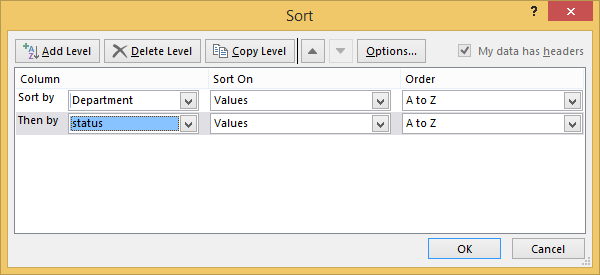
\includegraphics{./images/excel14.png}
\end{frame}

\begin{frame}{Filtrimi i Të Dhënave në Tabelë}
\phantomsection\label{filtrimi-i-tuxeb-dhuxebnave-nuxeb-tabeluxeb}
\begin{enumerate}
\item
  Klikoni mbi shigjetën në titullin e kolonës për të hapur menynë e
  filtrimit.
\item
  Zgjidhni vlerat që dëshironi të shfaqen duke përdorur kutizat e
  zgjedhjes.
\end{enumerate}
\end{frame}

\begin{frame}{Filtrimi i Të Dhënave në Tabelë}
\phantomsection\label{filtrimi-i-tuxeb-dhuxebnave-nuxeb-tabeluxeb-1}
\begin{enumerate}
\setcounter{enumi}{2}
\item
  Për filtrime të avancuara:

  \begin{itemize}
  \tightlist
  \item
    Zgjidhni \textbf{Number Filters} ose \textbf{Text Filters} për
    kritere specifike.
  \end{itemize}
\end{enumerate}

\textbf{Shembull}: Filtroni vetëm vlerat më të mëdha se 1000 në një
kolonë.

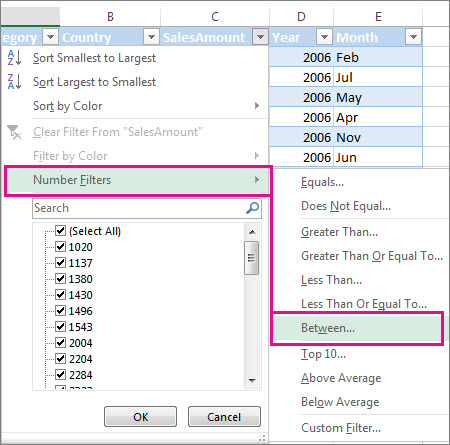
\includegraphics{./images/excel15.jpg}
\end{frame}

\begin{frame}{Shtimi i Totalëve në Tabelë}
\phantomsection\label{shtimi-i-totaluxebve-nuxeb-tabeluxeb}
\begin{enumerate}
\item
  Klikoni kudo brenda tabelës për ta aktivizuar.
\item
  Shkoni te \textbf{Table Design \textgreater{} Total Row} për të shtuar
  një rresht total.
\end{enumerate}
\end{frame}

\begin{frame}{Shtimi i Totalëve në Tabelë}
\phantomsection\label{shtimi-i-totaluxebve-nuxeb-tabeluxeb-1}
\begin{enumerate}
\setcounter{enumi}{2}
\item
  Në fund të tabelës, shtoni funksione si:

  \begin{itemize}
  \item
    \textbf{SUM}: Për të mbledhur vlera numerike.
  \item
    \textbf{AVERAGE}: Për të llogaritur mesataren.
  \item
    \textbf{COUNT}: Për të numëruar qelizat.
  \end{itemize}
\end{enumerate}
\end{frame}

\begin{frame}{Shtimi i Totalëve në Tabelë}
\phantomsection\label{shtimi-i-totaluxebve-nuxeb-tabeluxeb-2}
\textbf{Shembull}: Llogaritni totalin e shitjeve në një kolonë numerike.

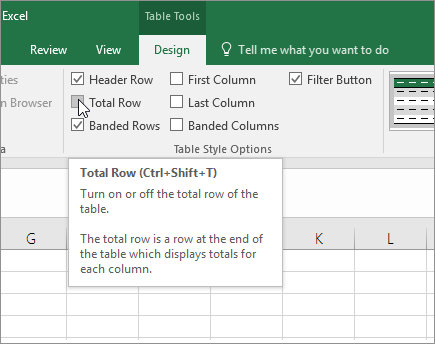
\includegraphics{./images/excel16.png}
\end{frame}

\begin{frame}{Përdorimi i Slicers për Filtrimin e Të Dhënave}
\phantomsection\label{puxebrdorimi-i-slicers-puxebr-filtrimin-e-tuxeb-dhuxebnave}
\textbf{Slicers} janë mjete vizuale për të filtruar të dhënat në tabelë.

\begin{enumerate}
\item
  Zgjidhni tabelën tuaj.
\item
  Shkoni te \textbf{Table Design \textgreater{} Insert Slicer}.
\end{enumerate}
\end{frame}

\begin{frame}{Përdorimi i Slicers për Filtrimin e Të Dhënave}
\phantomsection\label{puxebrdorimi-i-slicers-puxebr-filtrimin-e-tuxeb-dhuxebnave-1}
\begin{enumerate}
\setcounter{enumi}{2}
\item
  Zgjidhni kolonën që dëshironi të përdorni për filtrimin.
\item
  Përdorni \textbf{Slicer} për të filtruar të dhënat duke klikuar mbi
  vlerat e shfaqura.
\end{enumerate}
\end{frame}

\begin{frame}{Përdorimi i Slicers për Filtrimin e Të Dhënave}
\phantomsection\label{puxebrdorimi-i-slicers-puxebr-filtrimin-e-tuxeb-dhuxebnave-2}
\textbf{Shembull}: Filtroni të dhënat bazuar në një kategori të veçantë,
si ``Produktet''.
\end{frame}

\begin{frame}{Përfitimet e Përdorimit të Tabelave në Excel Web}
\phantomsection\label{puxebrfitimet-e-puxebrdorimit-tuxeb-tabelave-nuxeb-excel-web}
\begin{enumerate}
\item
  \textbf{Organizim më i mirë}: Tabelat krijojnë një strukturë të qartë
  për të dhënat.
\item
  \textbf{Analiza të shpejta}: Funksione si \textbf{Sort},
  \textbf{Filter}, dhe \textbf{Total} mundësojnë analiza të
  menjëhershme.
\end{enumerate}
\end{frame}

\begin{frame}{Krijimi i Një Grafiku nga Fillimi}
\phantomsection\label{krijimi-i-njuxeb-grafiku-nga-fillimi}
\begin{enumerate}
\item
  Zgjidhni të dhënat që dëshironi të vizualizoni.
\item
  Shkoni te \textbf{Insert \textgreater{} Chart} në Ribbon.
\end{enumerate}
\end{frame}

\begin{frame}{Krijimi i Një Grafiku nga Fillimi}
\phantomsection\label{krijimi-i-njuxeb-grafiku-nga-fillimi-1}
\begin{enumerate}
\setcounter{enumi}{2}
\item
  Zgjidhni llojin e grafikut:

  \begin{itemize}
  \item
    \textbf{Column} (Kolonë)
  \item
    \textbf{Line} (Vijë)
  \item
    \textbf{Pie} (Rrethor)
  \item
    \textbf{Bar}, \textbf{Scatter}, etj.
  \end{itemize}
\end{enumerate}
\end{frame}

\begin{frame}{Krijimi i Një Grafiku nga Fillimi}
\phantomsection\label{krijimi-i-njuxeb-grafiku-nga-fillimi-2}
\begin{enumerate}
\setcounter{enumi}{3}
\tightlist
\item
  Klikoni \textbf{OK} dhe grafiku juaj do të shfaqet në worksheet.
\end{enumerate}
\end{frame}

\begin{frame}{Shtimi ose Heqja e Titujve në Grafik}
\phantomsection\label{shtimi-ose-heqja-e-titujve-nuxeb-grafik}
\begin{enumerate}
\item
  Klikoni mbi grafikun për të aktivizuar opsionet e tij.
\item
  Zgjidhni \textbf{Chart Elements} (ikonë ``+'' pranë grafikut).
\end{enumerate}
\end{frame}

\begin{frame}{Shtimi ose Heqja e Titujve në Grafik}
\phantomsection\label{shtimi-ose-heqja-e-titujve-nuxeb-grafik-1}
\begin{enumerate}
\setcounter{enumi}{2}
\item
  Klikoni mbi \textbf{Chart Title} për të shtuar titullin.
\item
  Klikoni mbi titullin për të shkruar emrin e dëshiruar.
\end{enumerate}

\textbf{Heqja e titullit}: Hiqni shenjën pranë \textbf{Chart Title}.
\end{frame}

\begin{frame}{Shtimi ose Heqja e Legjendës dhe Tabelës së Të Dhënave}
\phantomsection\label{shtimi-ose-heqja-e-legjenduxebs-dhe-tabeluxebs-suxeb-tuxeb-dhuxebnave}
\begin{enumerate}
\item
  Klikoni mbi grafikun për të aktivizuar \textbf{Chart Elements}.
\item
  Zgjidhni:

  \begin{itemize}
  \item
    \textbf{Legend} për të shtuar ose fshehur legjendën.
  \item
    \textbf{Data Table} për të shfaqur tabelën e të dhënave nën
    grafikun.
  \end{itemize}
\end{enumerate}
\end{frame}

\begin{frame}{Shtimi i Një Boshti Dytësor}
\phantomsection\label{shtimi-i-njuxeb-boshti-dytuxebsor}
\begin{itemize}
\tightlist
\item
  Përdoret për të vizualizuar të dhëna me njësi ose vlera të ndryshme.
\end{itemize}

Hapat:

\begin{enumerate}
\item
  Klikoni mbi grafikun dhe zgjidhni një seri të dhënash që dëshironi të
  ndryshoni.
\item
  Klikoni me të djathtën dhe zgjidhni \textbf{Format Data Series}.
\end{enumerate}
\end{frame}

\begin{frame}{Shtimi i Një Boshti Dytësor}
\phantomsection\label{shtimi-i-njuxeb-boshti-dytuxebsor-1}
\begin{enumerate}
\setcounter{enumi}{2}
\item
  Zgjidhni \textbf{Secondary Axis} (Boshti Dytësor).
\item
  Excel do të shtojë boshtin në anën e djathtë të grafikut.
\end{enumerate}
\end{frame}

\begin{frame}{Shtimi i Një Linje Trendi ose Mesatare Lëvizëse}
\phantomsection\label{shtimi-i-njuxeb-linje-trendi-ose-mesatare-luxebvizuxebse}
\begin{enumerate}
\item
  Klikoni mbi grafikun dhe zgjidhni serinë e të dhënave.
\item
  Shkoni te \textbf{Chart Elements} dhe zgjidhni \textbf{Trendline}.
\end{enumerate}
\end{frame}

\begin{frame}{Shtimi i Një Linje Trendi ose Mesatare Lëvizëse}
\phantomsection\label{shtimi-i-njuxeb-linje-trendi-ose-mesatare-luxebvizuxebse-1}
\begin{enumerate}
\setcounter{enumi}{2}
\item
  Zgjidhni llojin e linjës së trendit:

  \begin{itemize}
  \item
    \textbf{Linear} për trend të drejtë.
  \item
    \textbf{Moving Average} për mesatare lëvizëse.
  \end{itemize}
\item
  Opsionale: Klikoni mbi linjën për të formatuar pamjen e saj.
\end{enumerate}
\end{frame}

\section{Microsoft 365 PowerPoint
Web}\label{microsoft-365-powerpoint-web}

\begin{frame}{Krijimi i Një Prezantimi të Ri}
\phantomsection\label{krijimi-i-njuxeb-prezantimi-tuxeb-ri}
\begin{enumerate}
\tightlist
\item
  Shkoni te \url{https://www.office.com} dhe identifikohuni me
  kredencialet tuaja.
\end{enumerate}
\end{frame}

\begin{frame}{Krijimi i Një Prezantimi të Ri}
\phantomsection\label{krijimi-i-njuxeb-prezantimi-tuxeb-ri-1}
\begin{enumerate}
\setcounter{enumi}{1}
\item
  Klikoni mbi \textbf{PowerPoint} për të hapur aplikacionin.
\item
  Zgjidhni:

  \begin{itemize}
  \item
    \textbf{New blank presentation} (Prezantim bosh).
  \item
    \textbf{Template} për të përdorur modele të gatshme.
  \end{itemize}
\end{enumerate}
\end{frame}

\begin{frame}{Krijimi i Një Prezantimi të Ri}
\phantomsection\label{krijimi-i-njuxeb-prezantimi-tuxeb-ri-2}
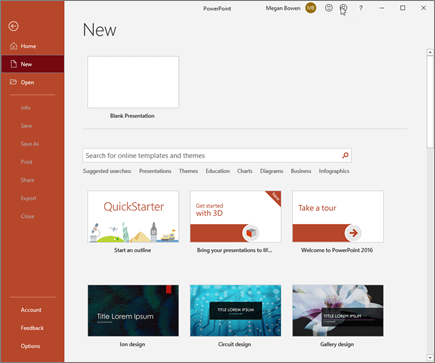
\includegraphics{./images/powerpoint1.png}
\end{frame}

\begin{frame}{Ruajtja e Prezantimit}
\phantomsection\label{ruajtja-e-prezantimit}
\begin{enumerate}
\item
  Prezantimi ruhet \textbf{automatikisht} në OneDrive gjatë punës.
\item
  Për ta ruajtur manualisht:

  \begin{itemize}
  \item
    Shkoni te \textbf{File \textgreater{} Save As}.
  \item
    Zgjidhni vendin dhe emrin për dokumentin.
  \end{itemize}
\end{enumerate}
\end{frame}

\begin{frame}{Ruajtja e Prezantimit}
\phantomsection\label{ruajtja-e-prezantimit-1}
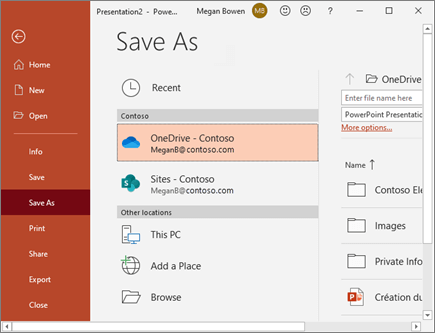
\includegraphics{./images/powerpoint2.png}
\end{frame}

\begin{frame}{Dizajnimi i Prezantimit}
\phantomsection\label{dizajnimi-i-prezantimit}
\begin{enumerate}
\item
  Shkoni te seksioni \textbf{Design} në Ribbon.
\item
  Zgjidhni një \textbf{tema} për të aplikuar një dizajn të paracaktuar.
\end{enumerate}
\end{frame}

\begin{frame}{Dizajnimi i Prezantimit}
\phantomsection\label{dizajnimi-i-prezantimit-1}
\begin{enumerate}
\setcounter{enumi}{2}
\item
  Për të ndryshuar \textbf{variacionin e ngjyrave}:

  \begin{itemize}
  \tightlist
  \item
    Klikoni mbi \textbf{Variants} dhe zgjidhni kombinimin e dëshiruar.
  \end{itemize}
\end{enumerate}

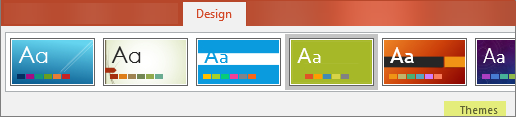
\includegraphics{./images/powerpoint3.png}
\end{frame}

\begin{frame}{Shtimi i Tekstit dhe Tabelave}
\phantomsection\label{shtimi-i-tekstit-dhe-tabelave}
\begin{enumerate}
\item
  Klikoni në një kuti teksti për të shtuar përmbajtjen.
\item
  Për të shtuar tabela:

  \begin{itemize}
  \tightlist
  \item
    Shkoni te \textbf{Insert \textgreater{} Table}.
  \end{itemize}
\end{enumerate}
\end{frame}

\begin{frame}{Shtimi i Tekstit dhe Tabelave}
\phantomsection\label{shtimi-i-tekstit-dhe-tabelave-1}
\begin{itemize}
\tightlist
\item
  Zgjidhni dimensionet e tabelës dhe plotësoni të dhënat.
\end{itemize}

\textbf{Këshillë}: Përdorni \textbf{Home \textgreater{} Font} për të
formatuar tekstin.
\end{frame}

\begin{frame}{Shtimi i Figurave dhe Grafikëve}
\phantomsection\label{shtimi-i-figurave-dhe-grafikuxebve}
\begin{enumerate}
\item
  Shkoni te \textbf{Insert} në Ribbon.
\item
  Shtoni elementë si:

  \begin{itemize}
  \item
    \textbf{Pictures} (Figurat) nga kompjuteri ose online.
  \item
    \textbf{Charts} për grafikë të të dhënave.
  \item
    \textbf{Icons} dhe \textbf{SmartArt} për ilustrime vizuale.
  \end{itemize}
\end{enumerate}
\end{frame}

\begin{frame}{Animacionet dhe Video/Audio}
\phantomsection\label{animacionet-dhe-videoaudio}
\begin{enumerate}
\item
  Shkoni te \textbf{Animations} për të shtuar efekte për tekstin ose
  objektet:

  \begin{itemize}
  \tightlist
  \item
    \textbf{Entrance} (Hyrje), \textbf{Emphasis} (Theksim),
    \textbf{Exit} (Dalje).
  \end{itemize}
\item
  Për të shtuar video ose audio:

  \begin{itemize}
  \item
    Shkoni te \textbf{Insert \textgreater{} Video} ose \textbf{Audio}.
  \item
    Ngarkoni skedarin ose përdorni burime online.
  \end{itemize}
\end{enumerate}
\end{frame}

\begin{frame}{Prezantimi i Slideshow-t}
\phantomsection\label{prezantimi-i-slideshow-t}
\begin{enumerate}
\item
  Shkoni te \textbf{Slide Show} në Ribbon.
\item
  Zgjidhni \textbf{From Beginning} për të filluar prezantimin nga
  fillimi.
\end{enumerate}
\end{frame}

\begin{frame}{Prezantimi i Slideshow-t}
\phantomsection\label{prezantimi-i-slideshow-t-1}
\begin{enumerate}
\setcounter{enumi}{2}
\tightlist
\item
  Përdorni shigjetat për të lëvizur midis slajdeve.
\end{enumerate}

\textbf{Këshillë}: Përdorni \textbf{Presenter View} për të parë shënimet
dhe kohën.
\end{frame}

\begin{frame}{Bashkëpunimi dhe Ndarja}
\phantomsection\label{bashkuxebpunimi-dhe-ndarja}
\begin{enumerate}
\item
  Klikoni mbi \textbf{Share} në të djathtë të ekranit.
\item
  Ftoni bashkëpunëtorët duke futur adresën e tyre të email-it.
\item
  Zgjidhni opsionin për lejet:

  \begin{itemize}
  \item
    \textbf{Can edit}: Lejo redaktimin.
  \item
    \textbf{Can view}: Vetëm për shikim.
  \end{itemize}
\end{enumerate}
\end{frame}

\end{document}
